\documentclass{article}

\usepackage[english]{babel}
\usepackage[margin=3cm]{geometry}
\usepackage{graphicx}
\usepackage{float}
\usepackage{caption}
\usepackage{hyperref}
\usepackage{amsmath}
\usepackage{wrapfig}
\usepackage[parfill]{parskip}

% fonts
\usepackage[T1]{fontenc}
\usepackage{helvet}
\renewcommand{\familydefault}{\sfdefault}

\graphicspath{{img/}}

% theorem environment
\usepackage{amssymb}

\newtheorem{theorem}{Definition}[section]

\usepackage{enumitem}

\newenvironment{thmenum}
 {\begin{enumerate}[label=\upshape\bfseries(\roman*)]}
 {\end{enumerate}}


% code
\usepackage{minted}
\setminted{frame=single,framesep=3pt,linenos}
\usepackage{upquote}
\usepackage{color}

\begin{document}

\begin{titlepage}
    \author{Tuur Vanhoutte}
    \title{Deep Learning}
\end{titlepage}

\pagenumbering{gobble}
\maketitle
\newpage
\tableofcontents
\newpage

\pagenumbering{arabic}

\section{Introduction to neural networks}

\begin{figure}[H]
    \centering
    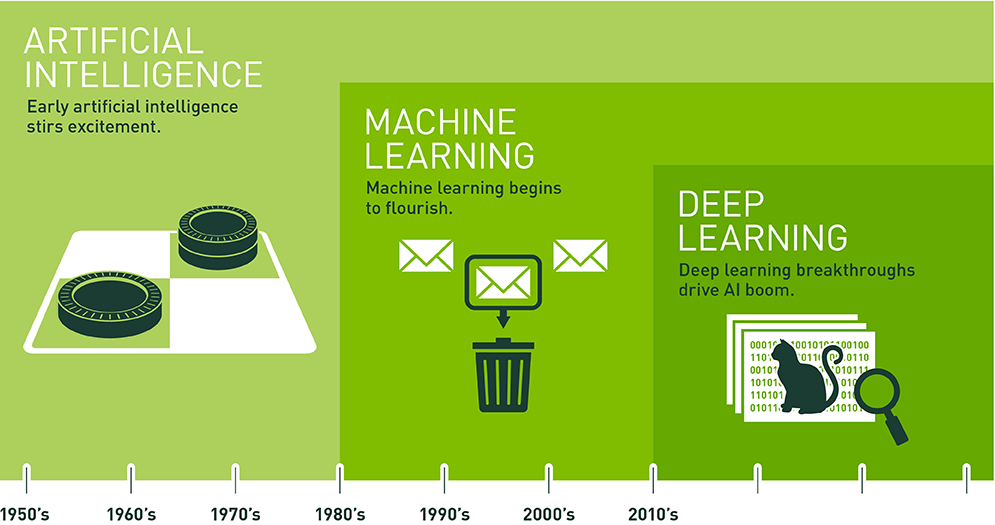
\includegraphics[width=0.6\textwidth]{ai-timeline.png}
    \caption{Timeline of AI}
\end{figure}

\subsection{Why deep learning?}

\begin{figure}[H]
    \centering
    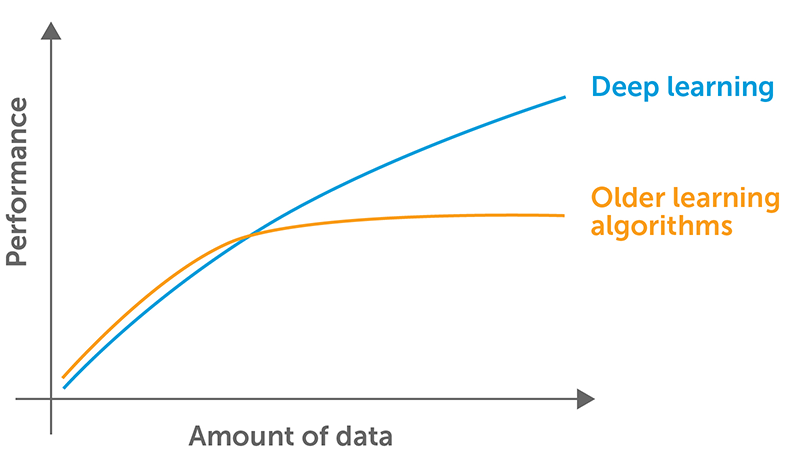
\includegraphics[width=0.5\textwidth]{deep-learning-performance-vs-data.png}
    \caption{Performance vs amount of data}
\end{figure}

\begin{itemize}
    \item The more data you have, the better the model
    \item In reality, older algorithms will plateau after a certain point
    \item With deep learning, this is much less of a problem
    \item However, neural networks are much more sensitive to overfitting: they can memorize the entire dataset
    \item For smaller datasets, it's often better to use traditional learning algorithms
\end{itemize}

\begin{figure}[H]
    \centering
    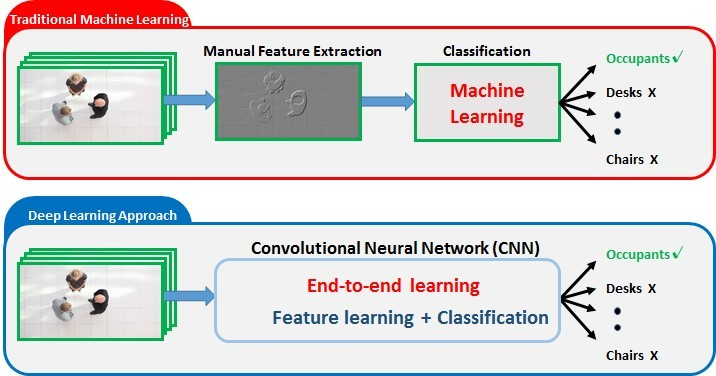
\includegraphics[width=0.7\textwidth]{deep-learning-approach.png}
    \caption{The difference in approach between traditional ML and Deep Learning}
\end{figure}

\begin{itemize}
    \item With traditional ML, you first need to extract the features manually 
    \item In the past, you had to manually mark facial features for facial recognition algorithms (eyes, mouth, ears, \dots)
    \item Deep learning is great for problems with non-structured data
    \begin{itemize}
        \item Structured data = rows of data (like an Excel-sheet)
        \item Non-structured = images, video, audio
    \end{itemize}
\end{itemize}

\begin{theorem}
    End-to-end learning is a deep learning technique where we run all raw data through a neural network.
    The neural network will do its own feature extraction (feature learning), and then a classifier will output predictions.
\end{theorem}


\subsection{The neural network}

\begin{figure}[H]
    \centering
    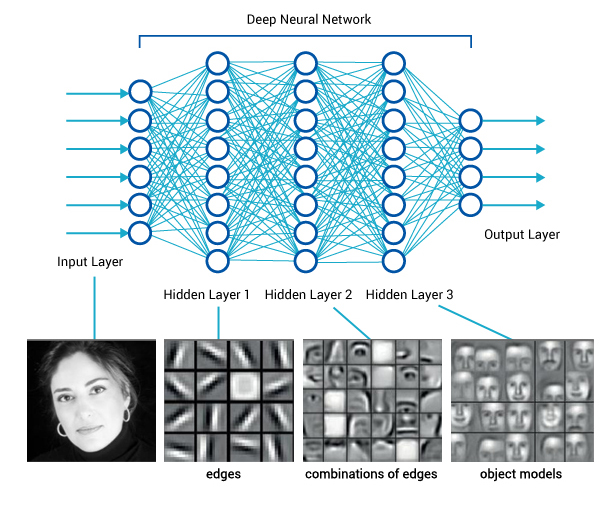
\includegraphics[width=0.5\textwidth]{neuraal-netwerk.png}
\end{figure}

\begin{itemize}
    \item The neurons are in one of three layers:
    \begin{itemize}
        \item Input layer
        \item Hidden layers
        \item Output layer
    \end{itemize}
    \item Every neuron is connected to every neuron of the next layer
    \item Every connection has a weight
    \item Deep Neural network $\Leftrightarrow$ multiple hidden layers
\end{itemize}

\subsection{History of deep learning}

\begin{figure}[H]
    \centering
    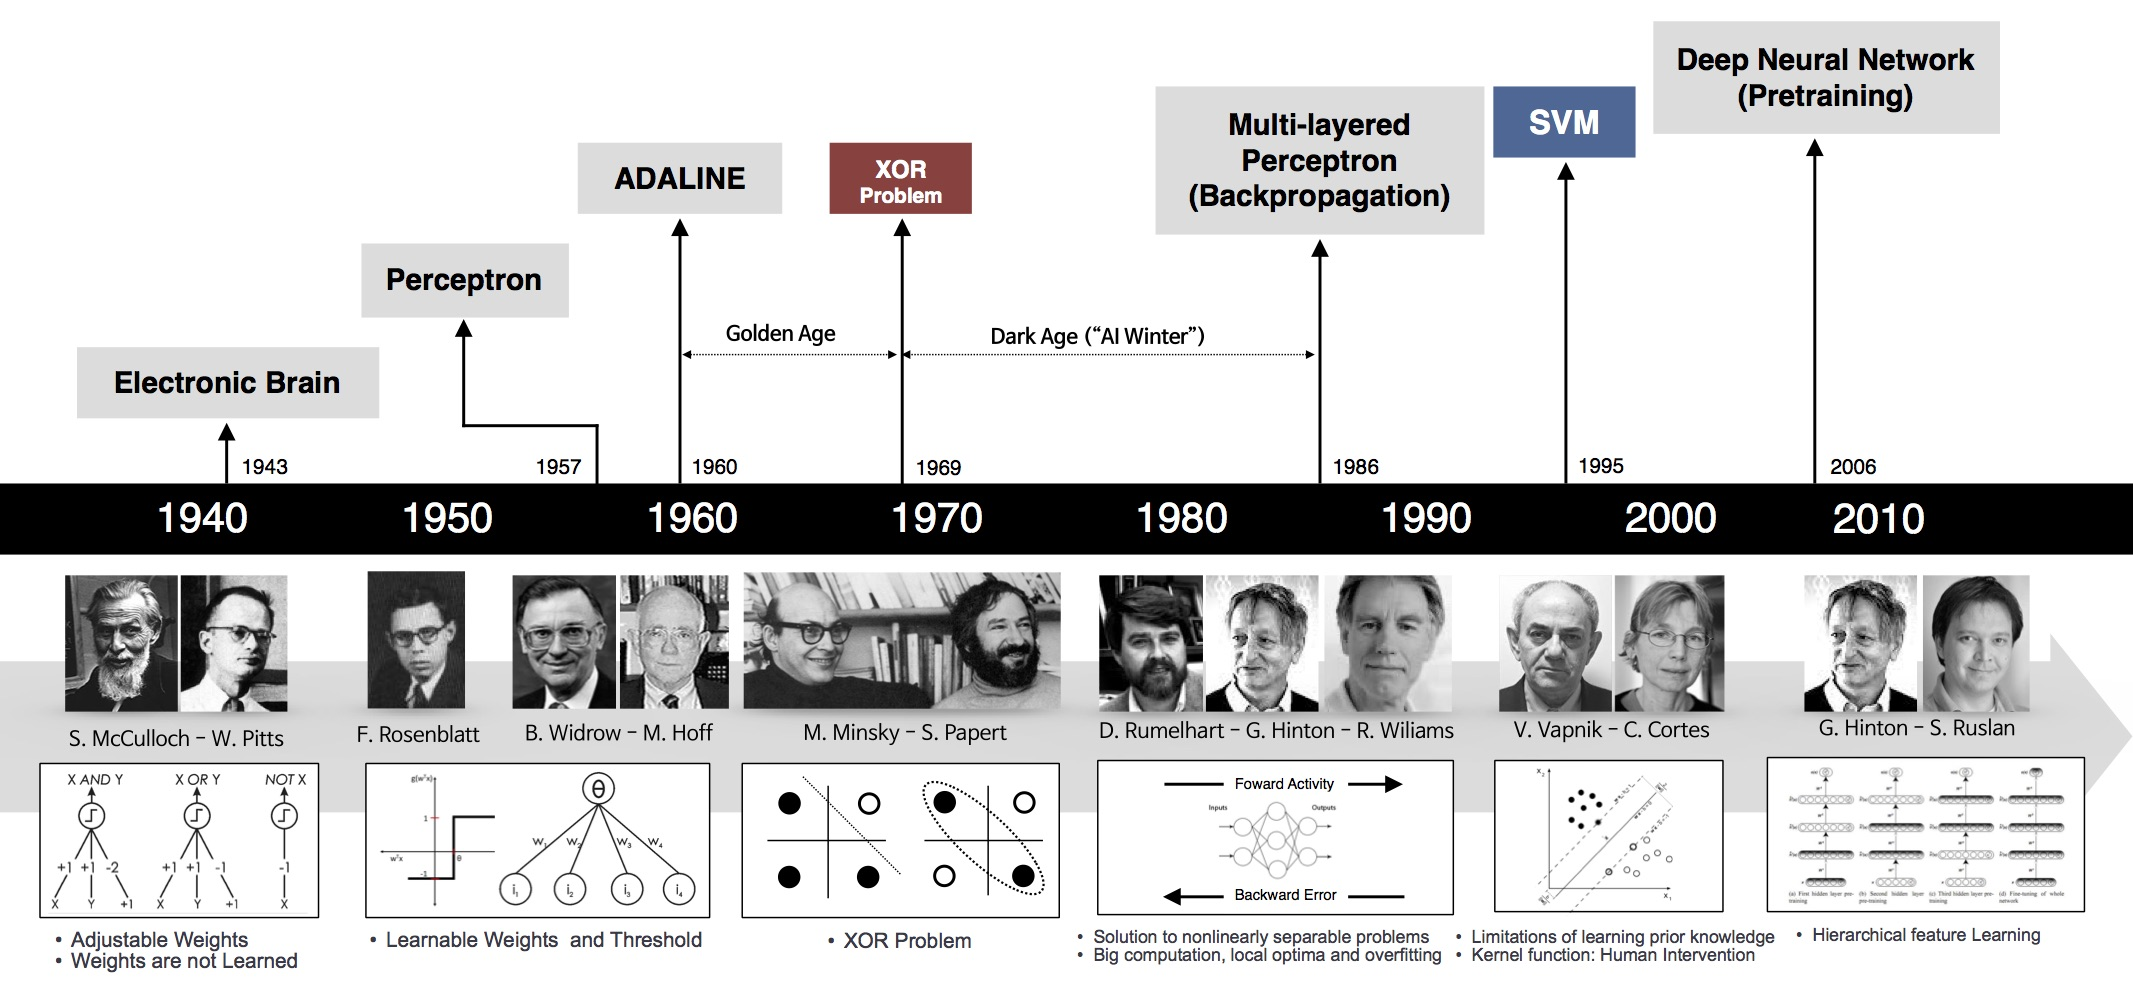
\includegraphics[width=0.5\textwidth]{deep-learning-history.png}
    \caption{\url{https://beamandrew.github.io/deeplearning/2017/02/23/deep_learning_101_part1.html}}
\end{figure}


\subsection{Deep learning architectures}

You can change many things about the components of a neural network. 
Here are some examples of popular architectures. The most important ones are in \textbf{bold}:

\begin{itemize}
    \item \textbf{Convolutional Neural Networks (CNN)}
    \item Capsule Network (CapsNet)
    \item Restricted Boltzmann Machine (RBM)
    \item \textbf{Autoencoder (AE)}
    \item Deep Belief Nets (DBN)
    \item \textbf{Recurrent Neural (Tensor) Network (RNTN)}
    \item \textbf{Long Short Term Memory (LSTM)}
    \item \textbf{Gated Recurrent Unit nets (GRU)}
    \item \textbf{Generatative Adversarial Nets (GAN)}
    \item \dots
\end{itemize}

\subsection{Biological model}

\begin{figure}[H]
    \centering
    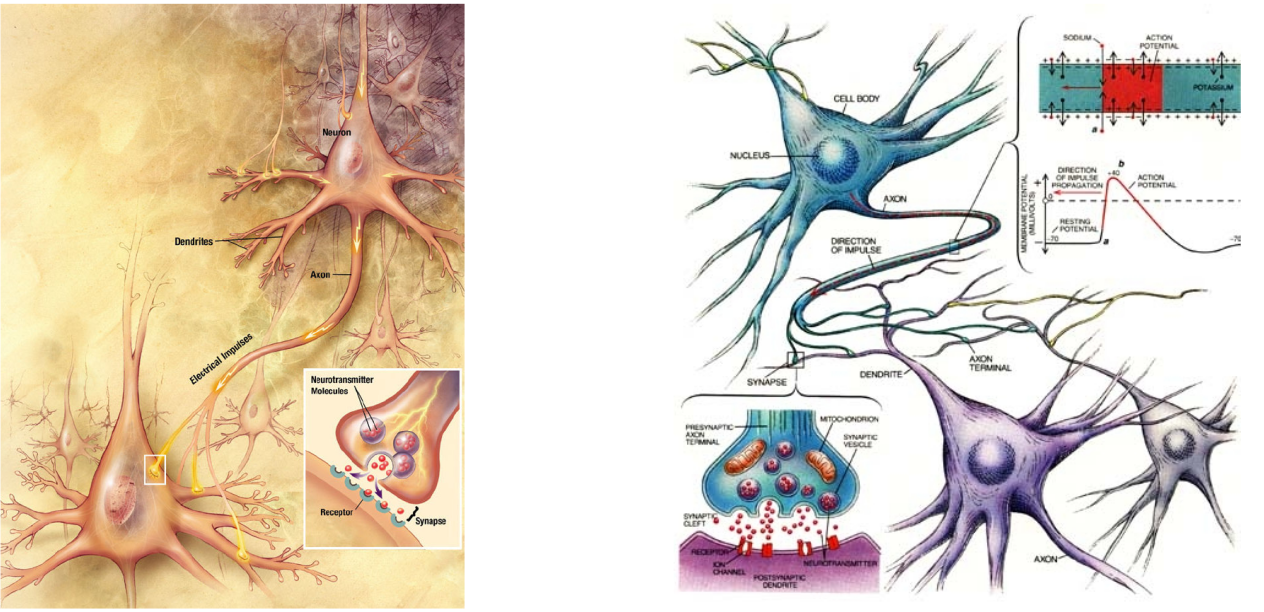
\includegraphics[width=0.5\textwidth]{biologisch-neuron.png}
    \caption{Anatomy of a biological neuron}
\end{figure}

\begin{itemize}
    \item Neural networks are inspired by our brains
    \item A neuron has multiple connections that can send signals to other neurons
    \item A neuron can send a weak or strong signal
\end{itemize}

\subsection{The artificial neuron}

\begin{figure}[H]
    \centering
    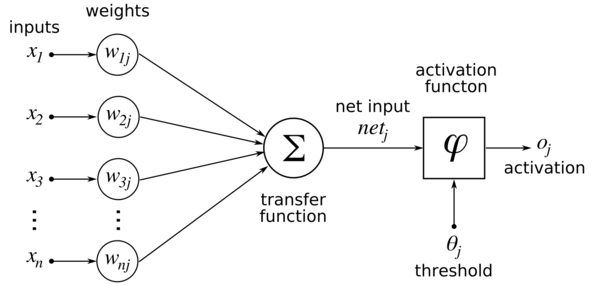
\includegraphics[width=0.5\textwidth]{neuron.png}
    \caption{Conceptual model}
\end{figure}

\begin{itemize}
    \item A neuron can receive multiple inputs
    \item Every input has a specified weight (= weak or strong signal)
    \item These inputs are multiplied by the weights, to then be used in a transfer function
    \item The transfer function is a mathematical formula that has a number as output
    \item That number is used as an input by an activation function. This functin will determine the final output
    \item \url{https://en.wikipedia.org/wiki/Activation_function}
\end{itemize}

\begin{figure}[H]
    \centering
    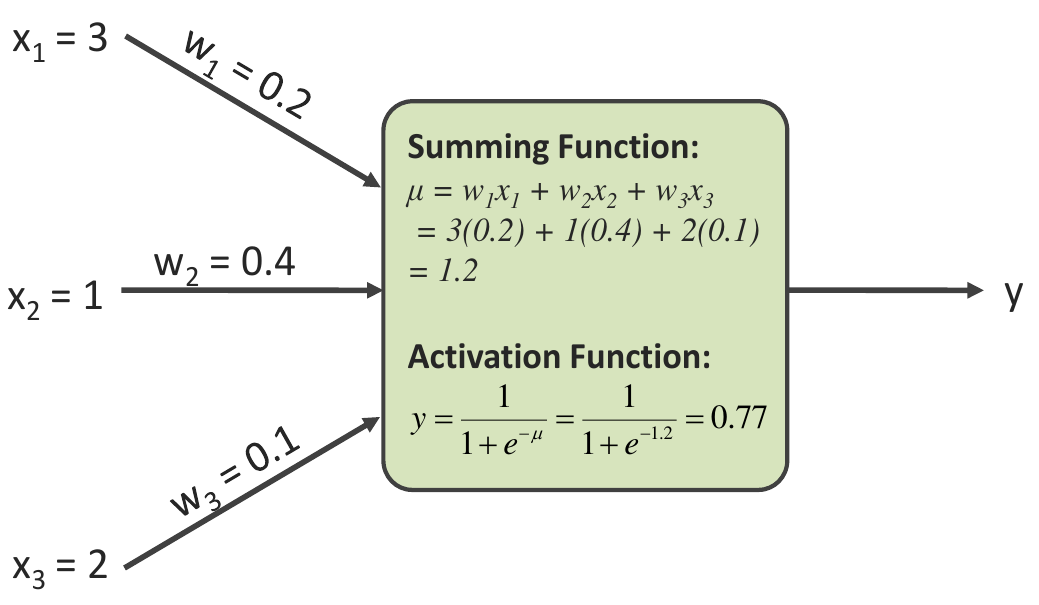
\includegraphics[width=0.5\textwidth]{neuron-voorbeeld.png}
    \caption{Example of a neuron, with a sigmoid function as activation function}
\end{figure}

\section{Logistic Regression}

\begin{theorem}
    Logistic regression is used to determine the probability of a certain sample 
    belonging to one of two classes.
    
    The name is a bit misleading: Logistic Regression is a classification technique, not regression. 
    The reason for this name is because regression is used to calculate the classification.
\end{theorem}

\subsection{The model}

Because the output is a probability, we're looking for a function $h_w$ so the model $h_w(x)$ :

\begin{center}
$0 \leq h_w(x) \leq 1$
\end{center}

\begin{itemize}
    \item $h_w(x)$ = estimated probability that $y=1$ for input $x$
    \item Example: $h_w(x) = 0.80$
    \begin{itemize}
        \item The model is 80\% sure that the sample belongs to class 1
        \item If you use a threshold of 50\%, the model will output 1
        \item If the prediction is less than that threshold of 50\%, the model will output 0
    \end{itemize}
\end{itemize}

\subsubsection{The logistic function}

\begin{equation}
h_w(x) = \frac{1}{1 + e^{-w^{\tau}x}}
\end{equation}

\begin{itemize}
    \item With $e =$ Euler's number = $\approx 2.718$
    \item This is a sigmoid function: the basic form for this is $\frac{1}{1+e^{-z}}$
    \item In our logistic function, $z$ equals $w^{\tau}x$
    \begin{itemize}
        \item This is equal to the solution of a linear regression function
        \item With $x =$ the sample values
        \item With $w =$ the weights that correspond to those values 
    \end{itemize}
\end{itemize}

\begin{figure}[H]
    \centering
    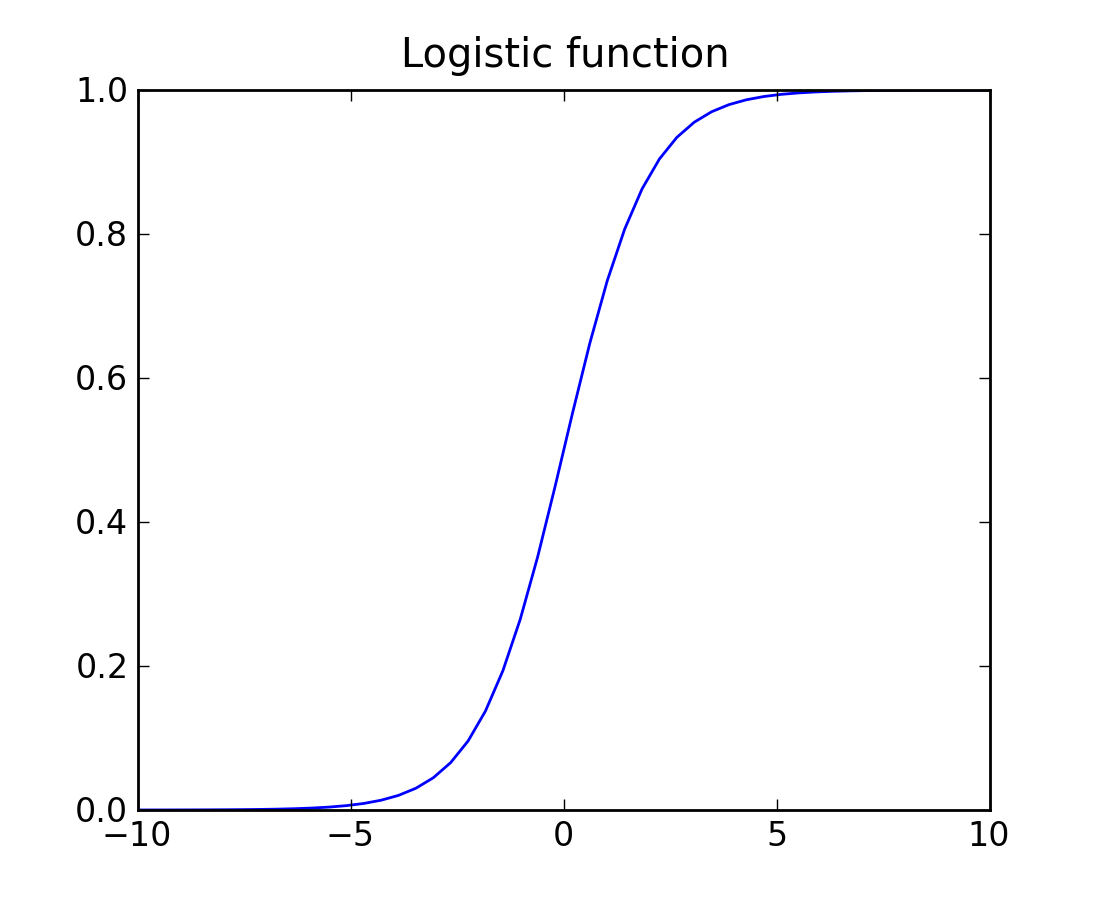
\includegraphics[width=0.3\textwidth]{logistic-regression.png}
    \caption{The logistic functie is evidently a sigmoid function or `S-function'}
\end{figure}

\begin{itemize}
    \item $y=1$ als $h_w(x) \geq 0.5 \Rightarrow w^{\tau}x \geq 0$
    \item $y=0$ als $h_w(x) < 0.5 \Rightarrow w^{\tau}x < 0$
\end{itemize}

\begin{figure}[H]
    \centering
    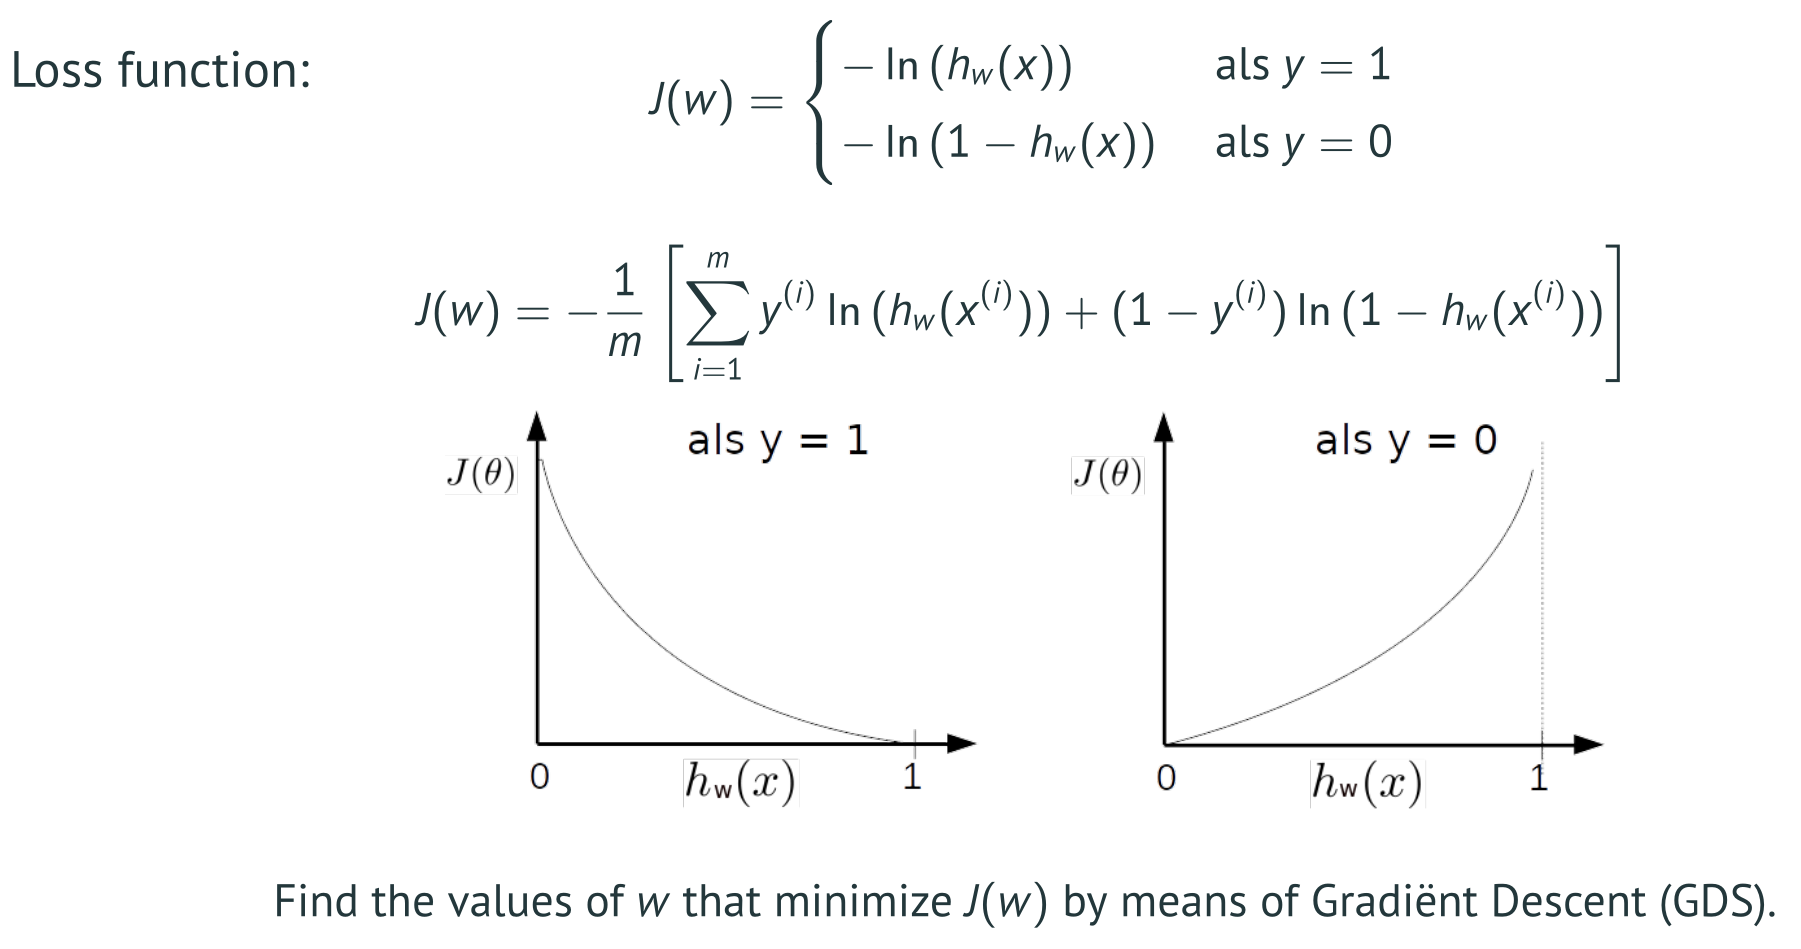
\includegraphics[width=0.5\textwidth]{img/logistic-regression-loss.png}
    \caption{Minizing the binary cross-Entropy loss function}
\end{figure}


\subsection{Logistic regression as a neuron}

\begin{figure}[H]
    \centering
    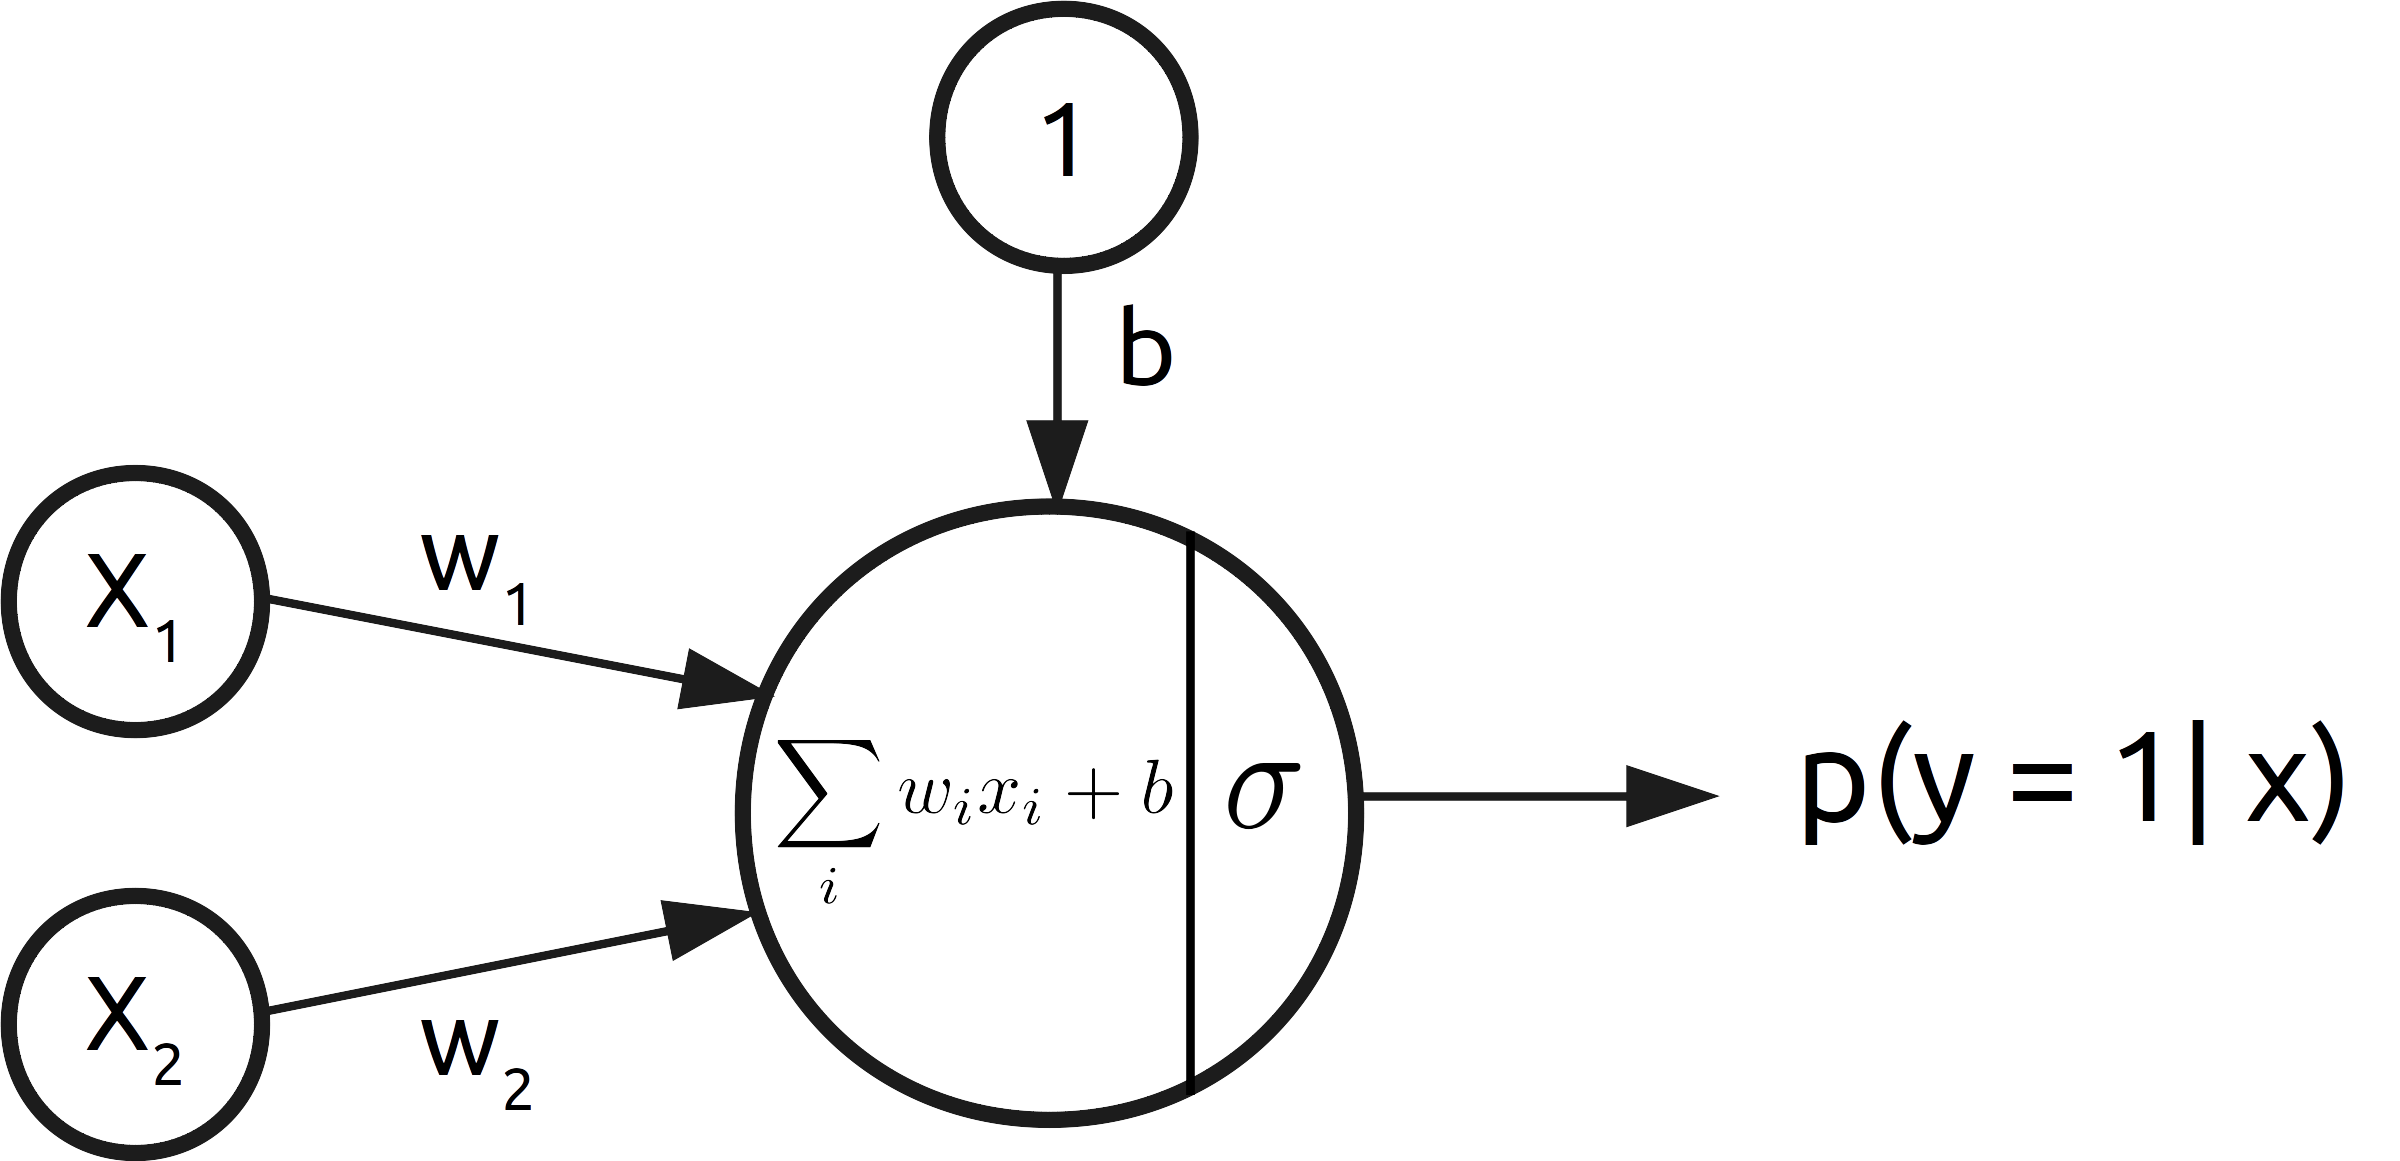
\includegraphics[width=0.5\textwidth]{logistic-regression-neuron.png}
    \caption{Logistic regression as a neuron}
\end{figure}

\subsubsection{Example}

\begin{figure}[H]
    \centering
    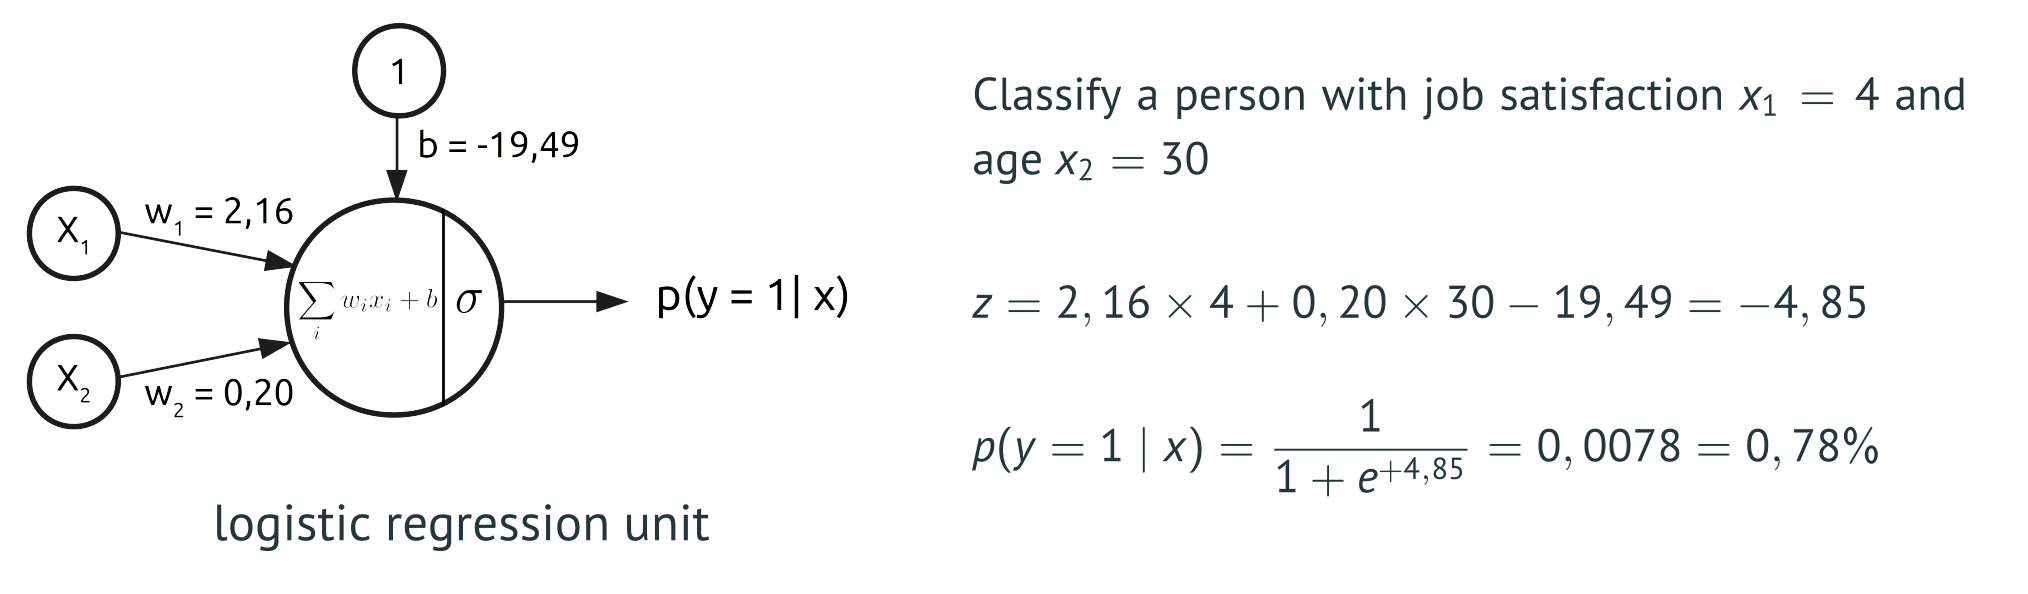
\includegraphics[width=0.75\textwidth]{img/logistic-regression-neuron-example.png}
\end{figure}

\begin{figure}[H]
    \centering
    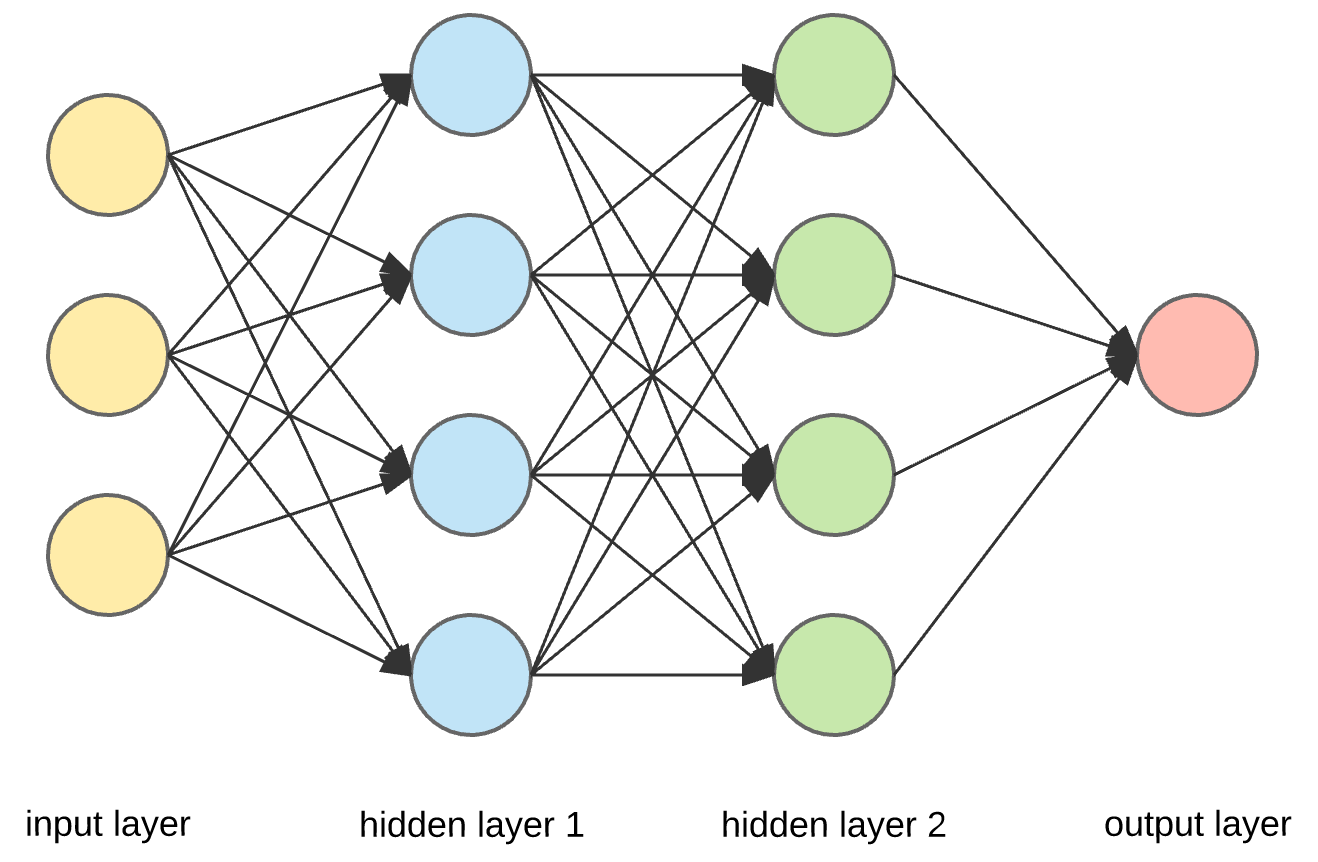
\includegraphics[width=0.5\textwidth]{img/neural-network-logistic-regression-units.png}
    \caption{A neural network can be modeled as a network of logistic regression units.}
\end{figure}

\subsection{Logistic regression vs neural networks}

In case of non-linearly separable data:

\begin{itemize}
    \item Use higher order features
    \item Neural networks make new representations of existing features.
\end{itemize}


\subsubsection{Example}

\begin{figure}[H]
    \centering
    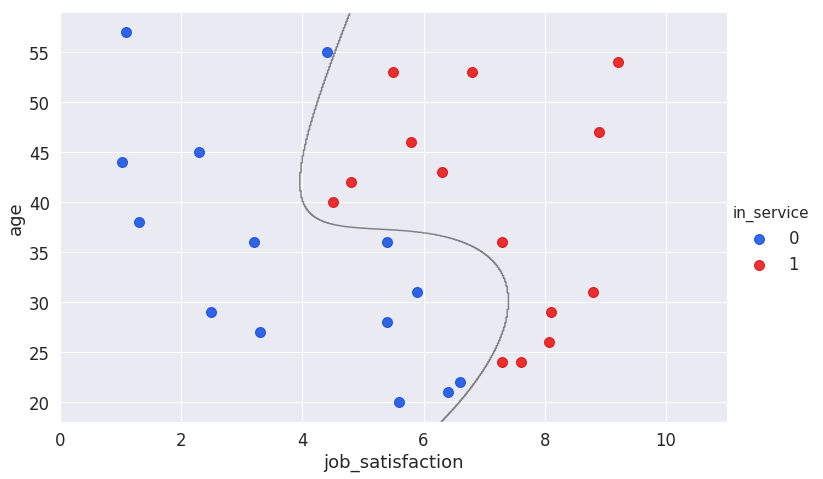
\includegraphics[width=0.6\textwidth]{img/decision-boundary-logreg.png}
    \caption{Decision boundary using 3rd order features with logistic regression}
\end{figure}

\begin{figure}[H]
    \centering
    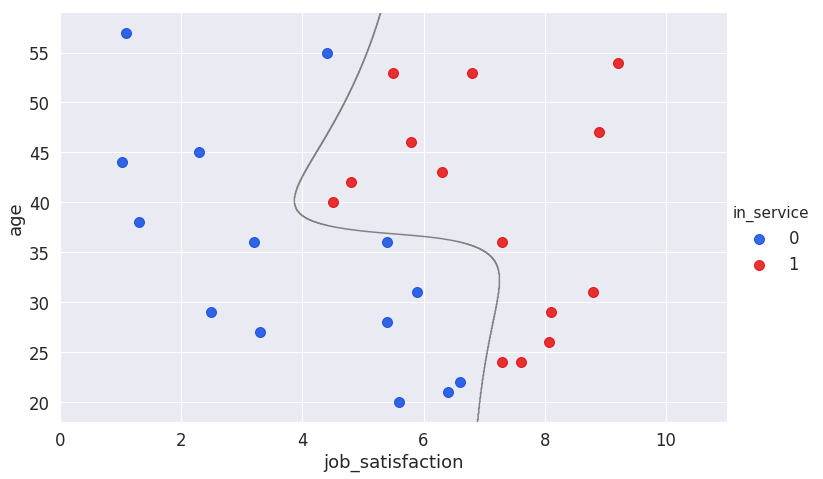
\includegraphics[width=0.6\textwidth]{img/decision-boundary-nn.png}
    \caption{Decision boundary of a neural network}
\end{figure}


\begin{figure}[H]
    \centering
    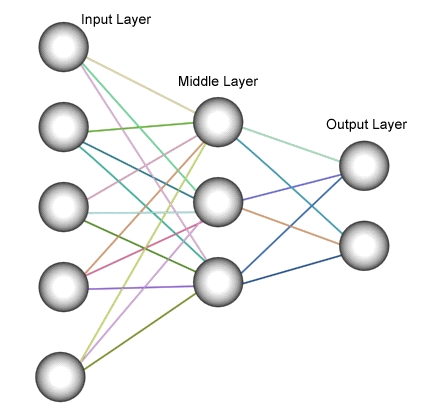
\includegraphics[width=0.3\textwidth]{img/properties-nn.png}
\end{figure}


\section{Basics of a neural network}
\subsection{Properties of a neural network}

\begin{itemize}
    \item Network architecture
    \item Learning algorithm
    \item Activation functions
\end{itemize}

You want the neural network to adapt and generalize to the data.

\subsubsection{Common network architectures}

\begin{figure}[H]
    \centering
    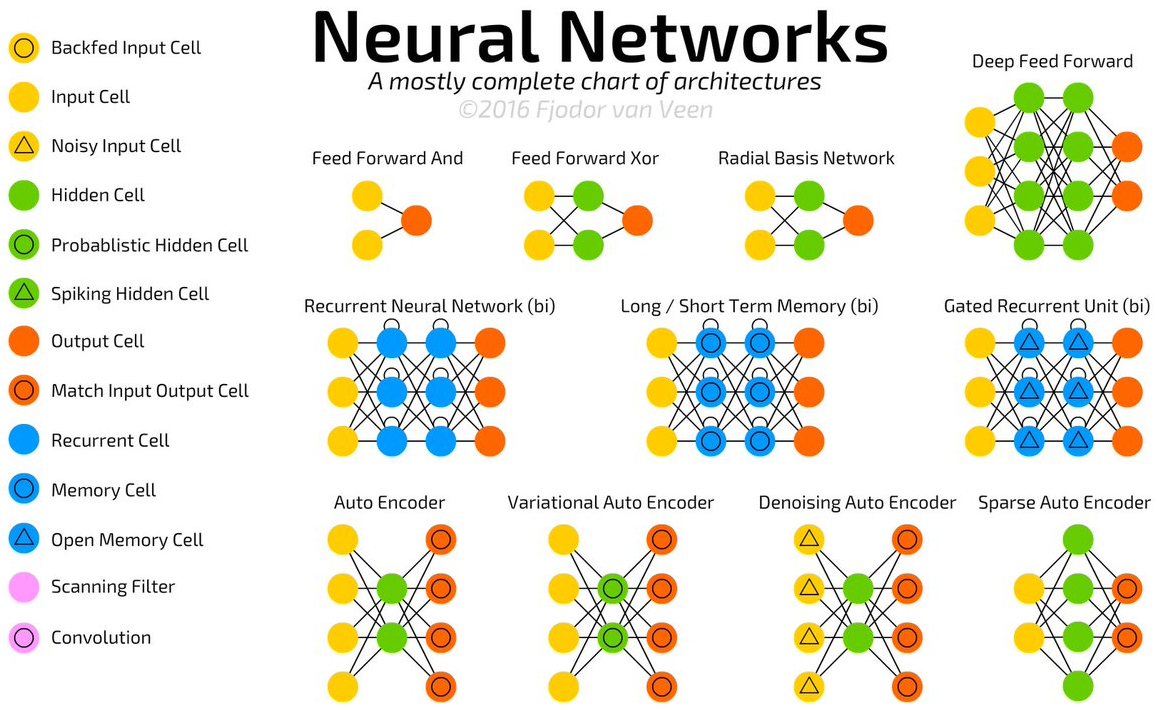
\includegraphics[width=0.6\textwidth]{img/network-architectures.png}
    \caption{\url{http://www.asimovinstitute.org/neural-network-zoo/}}
\end{figure}

\subsection{Feedforward neural networks}

\subsubsection{Properties}

\begin{itemize}
    \item 1 or more (hidden) layers.
    \item Each neuron is in a layer is connected to every neuron in the next layer.
    \item Signals travel from input to output through the hidden layers. (feedforward)
    \item The neural network maps inputs to desired outputs.
\end{itemize}


\begin{figure}[H]
    \centering
    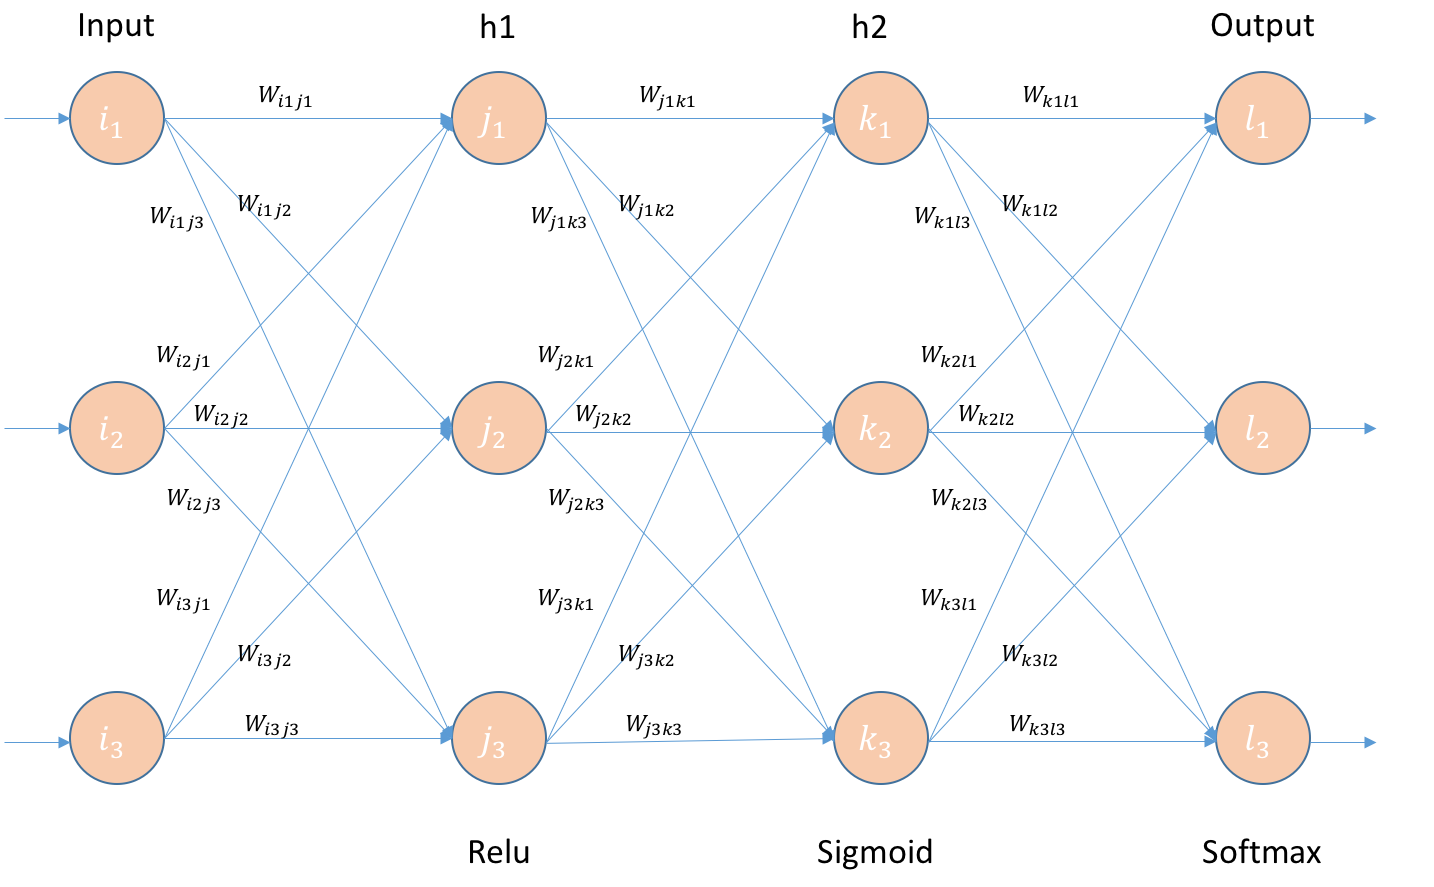
\includegraphics[width=0.5\textwidth]{feedforward-neural-network-properties.png}
    \caption{Feedforward neural network architecture}
\end{figure}

\subsubsection{MNIST example}

\begin{figure}[H]
    \centering
    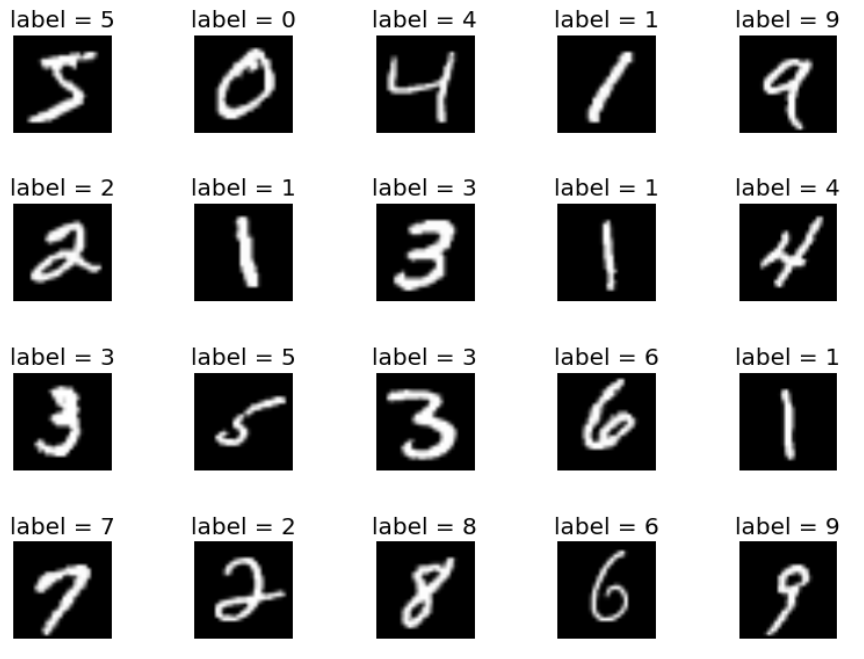
\includegraphics[width=0.4\textwidth]{mnist-neural.png}
    \caption{MNIST: dataset with labeled, handdrawn numbers}
\end{figure}

\begin{figure}[H]
    \centering
    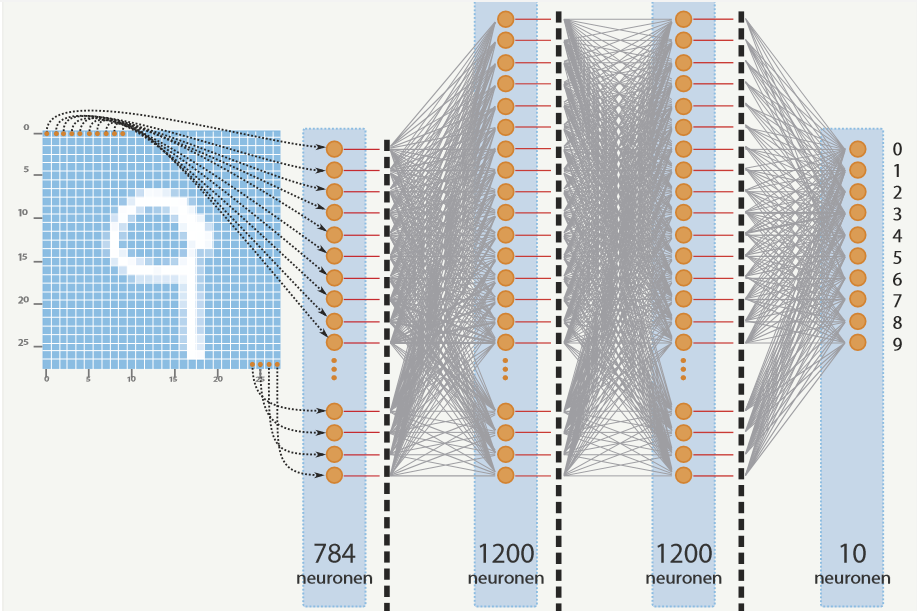
\includegraphics[width=0.5\textwidth]{mnist-neural2.png}
    \caption{Simplified example of a neural network}
\end{figure}

\begin{itemize}
    \item The numbers are drawn on a 28x28 grid (=784 input neurons)
    \item Every output (0-9) has a certain chance
    \item That chance determines how certain the model is that the given input is that number
    \item The chance is calculated using \textbf{backpropagation} (see later)
\end{itemize}

\subsubsection{One-hot encoding}

\begin{theorem}
    One-hot encoding is a technique to transform categorical features or targets to a more suitable format. 
    In a one-hot encoded target vector, the index of 1 represents the target label. All other values are 0.

    This is also used in neural networks.
\end{theorem}

\begin{figure}[H]
    \centering
    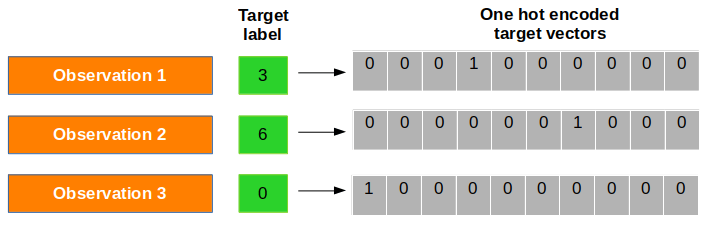
\includegraphics[width=0.4\textwidth]{one-hot.png}
\end{figure}

\begin{figure}[H]
    \centering
    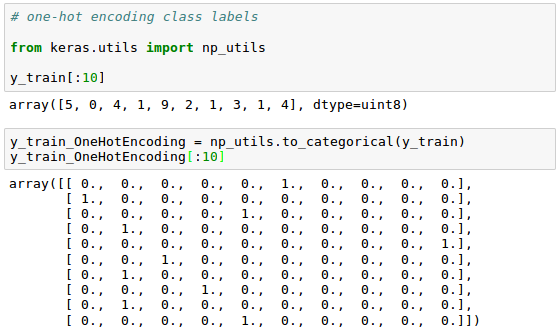
\includegraphics[width=0.5\textwidth]{one-hot2.png}
    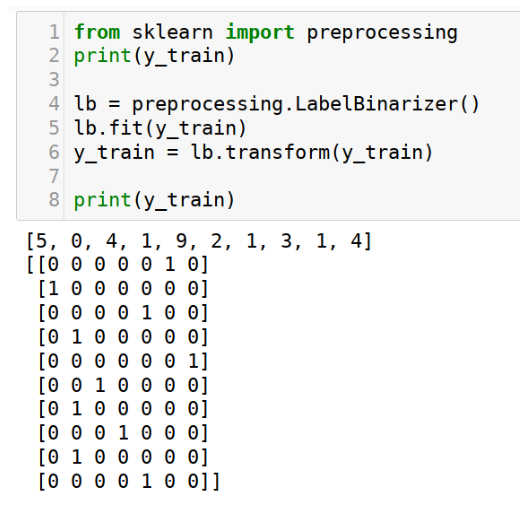
\includegraphics[width=0.3\textwidth]{neural-onehot.png}
    \caption{}
\end{figure}

\subsection{Multiclass classification}


How to classify with more than 2 classes?

\begin{figure}[H]
    \centering
    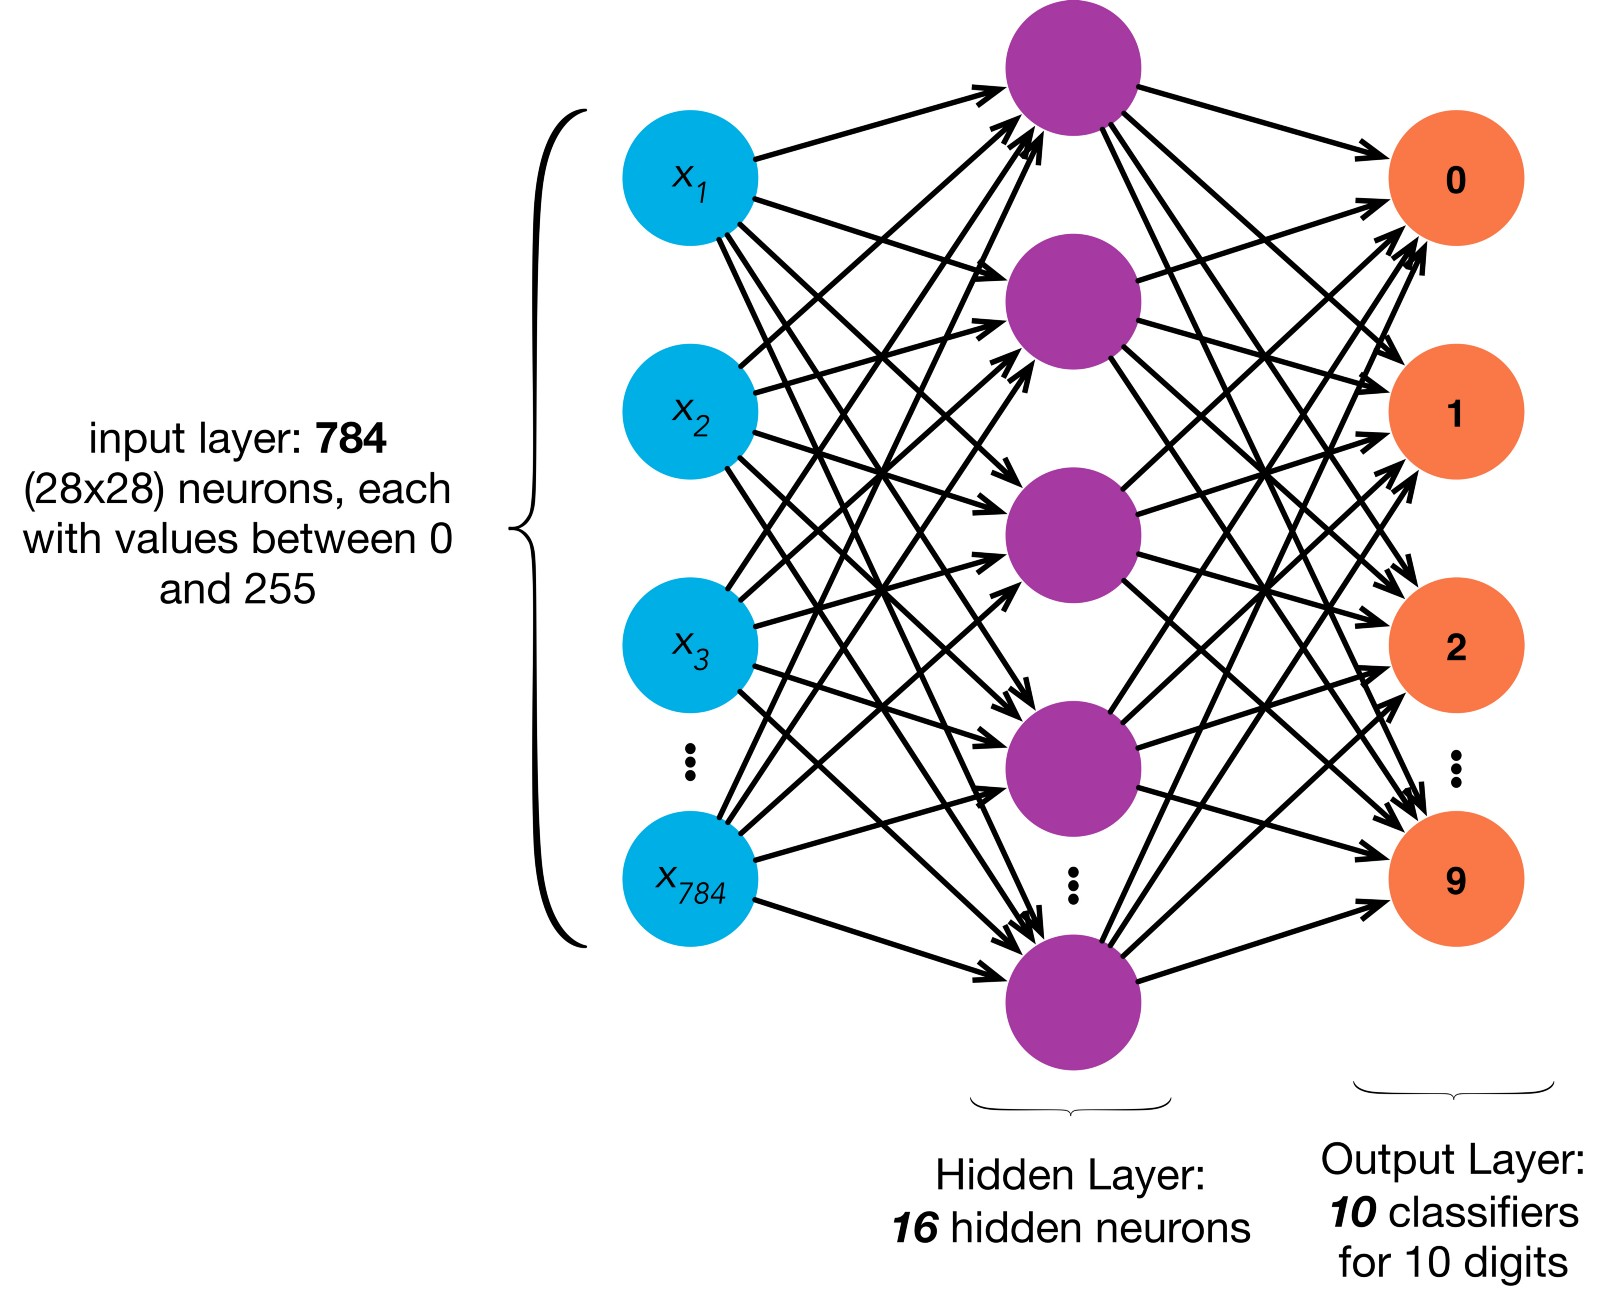
\includegraphics[width=0.5\textwidth]{multiclass-classification.png}
    \caption{}
\end{figure}

\begin{itemize}
    \item Sigmoid functions only allow for binary classification 
    \item We need a different function for multiclass classification with $K$ classes
    \item $\Rightarrow$ \textbf{Softmax function}
\end{itemize}

\begin{figure}[H]
    \centering
    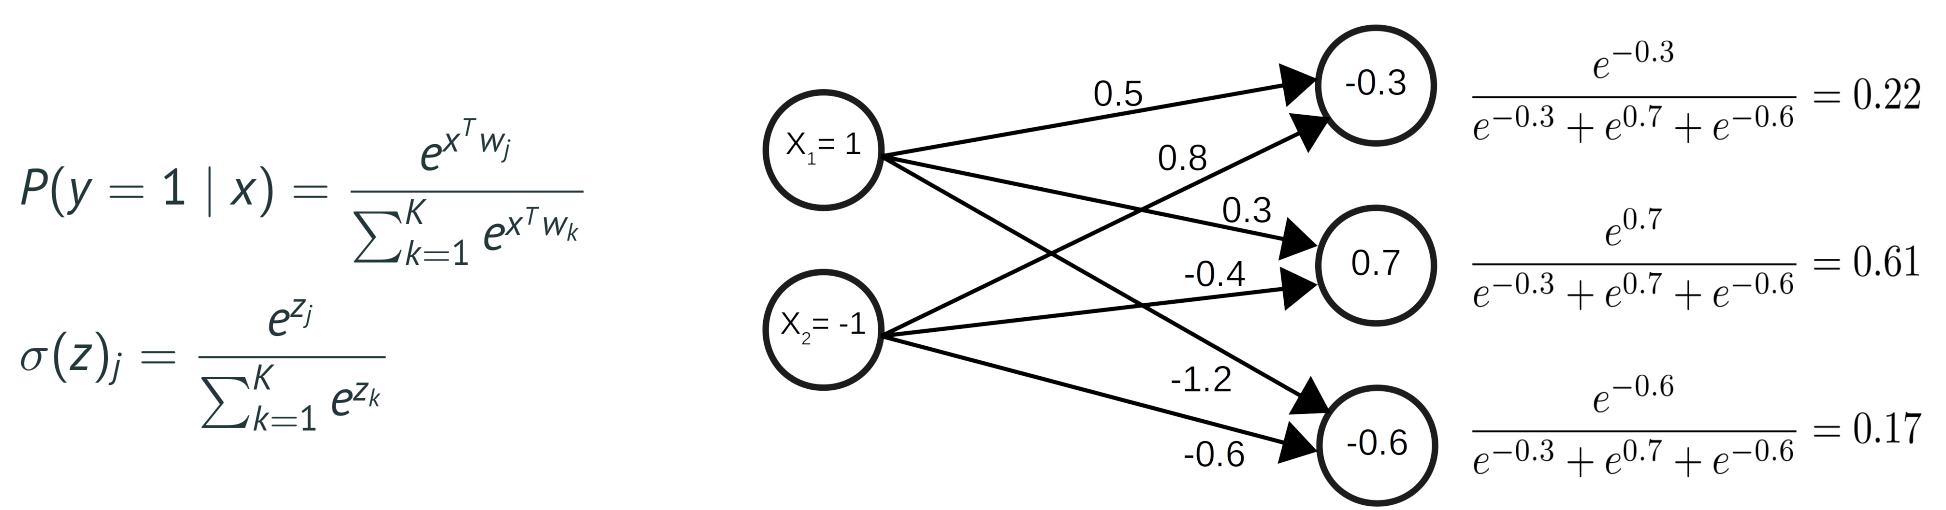
\includegraphics[width=0.85\textwidth]{img/softmax.png}
    \caption{Softmax function}
\end{figure}

TODO: more info about softmax

\begin{figure}[H]
    \centering
    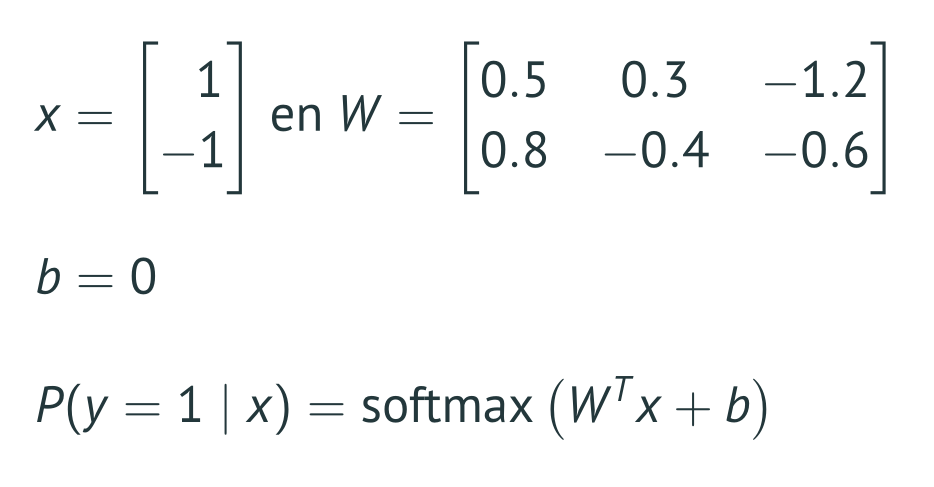
\includegraphics[width=0.5\textwidth]{img/softmax2.png}
    \caption{Output computation in vector notation}
\end{figure}


\subsubsection{Backpropagation}

\begin{theorem}
    Backpropagation is the most popular technique to train neural networks.
    It works by calculating an error (=loss) for every prediction, and to adjust the weights based on that error.
    
    The goal is to decrease the error as much as possible.
\end{theorem}

\begin{figure}[H]
    \centering
    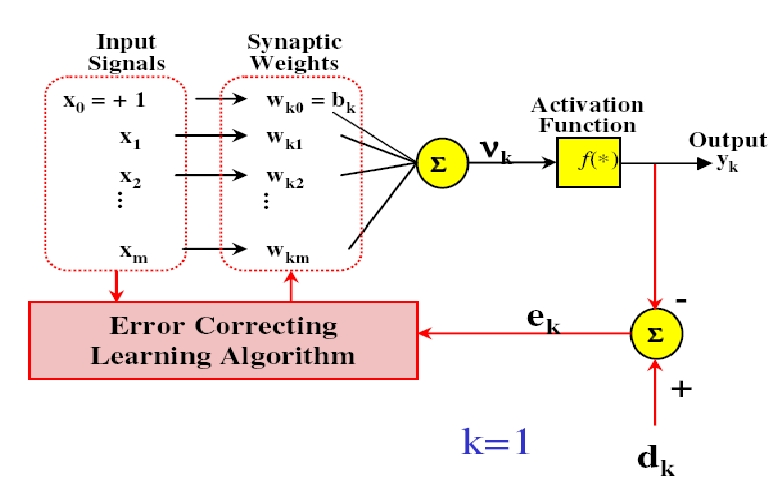
\includegraphics[width=0.5\textwidth]{img/backpropagation.png}
    \caption{}
\end{figure}

\begin{itemize}
    \item $\eta$ is the learning rate
    \item $0 < m \cdot \eta < 1$ with $m$ the number of inputs
    \item Error: $e_k(n) = d_k(n) - y_k(n)$
    \begin{itemize}
        \item Minimize the error $e_k(n)$
        \item $\epsilon(n) = \frac12 \sum_k e^2_k(n)$
        \item $\Delta W_{kj}(n) = \eta \cdot e_k(n) \cdot x_j(n)$
        \item Adjust the weight: $\Delta W_{kj}(n+1) = W_{kj}(n) + \Delta W_{kj}(n)$
    \end{itemize}
\end{itemize}

\url{https://becominghuman.ai/back-propagation-is-very-simple-who-made-it-complicated-97b794c97e5c}

\textbf{Using the MNIST example:}

\begin{itemize}
    \item In the output layer, the neural network assigns a probability to every number
    \item The prediction is made based on the highest chance.
    \item Suppose a certain number received too high a probability, and the true number too low a probability:
    \begin{itemize}
        \item The neural network will calculate the differences (=error)
        \item Next time, the neural network will try to keep the error as low as possible
        \item It does this by repeatedly adjusting the weights
        \item This process happens through all layers, from back to front $\Rightarrow$ \textbf{backpropagation}
    \end{itemize}
\end{itemize}

\begin{figure}[H]
    \centering
    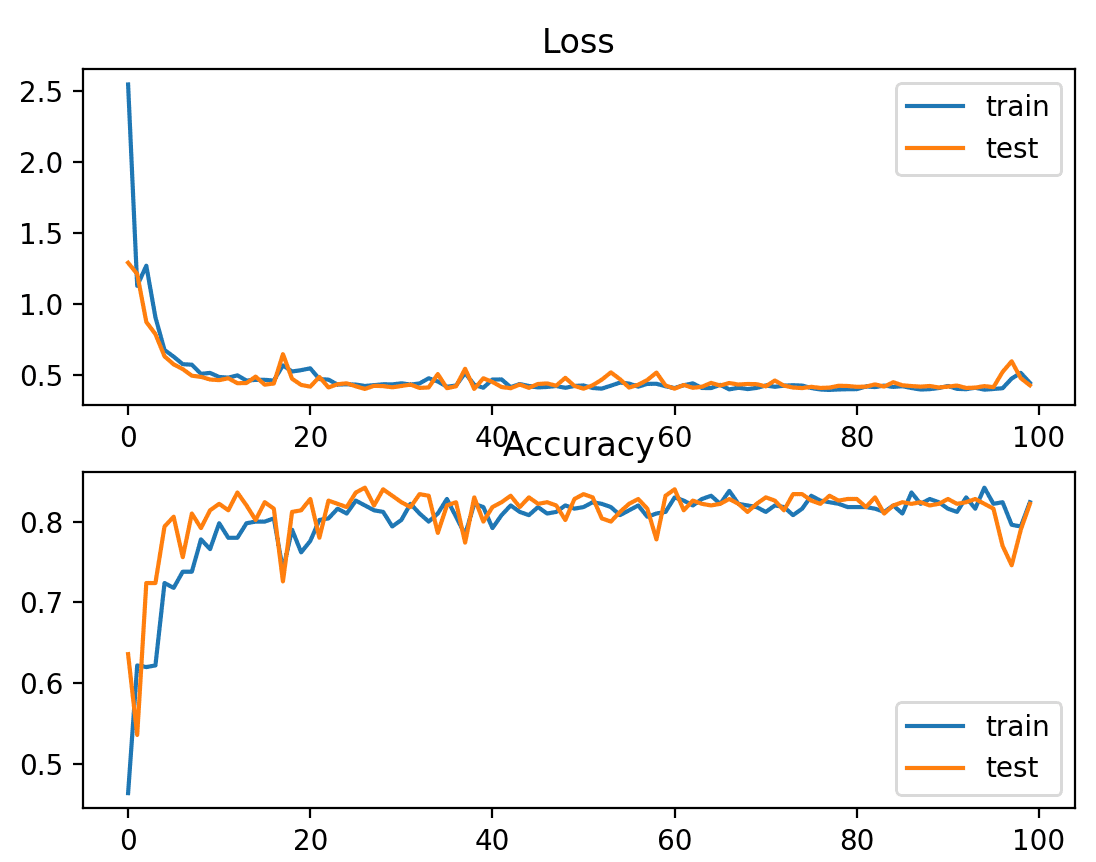
\includegraphics[width=0.5\textwidth]{backpropagation-error.png}
    \caption{The error function (=loss) in function of the amount of training epochs}
\end{figure}


\begin{figure}[H]
    \centering
    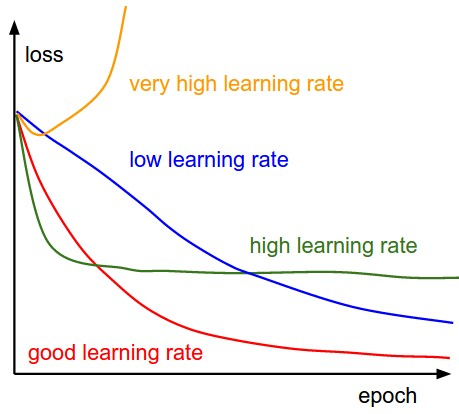
\includegraphics[width=0.4\textwidth]{backpropagation-learning-rate.png}
    \caption{Impact of the learning rate on the loss. During training, the learning rate keeps changing.}
\end{figure}

\subsection{Activation function}

\begin{figure}[H]
    \centering
    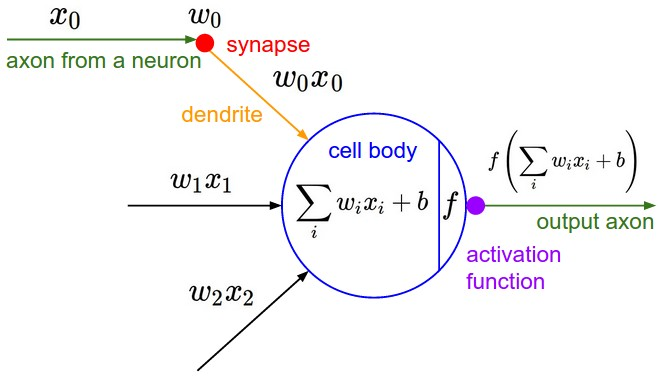
\includegraphics[width=0.5\textwidth]{activation-function.png}
\end{figure}


\begin{theorem}
    The activation function of a neuron defines the output of that neuron using a mathematical function.
    The inputs are multiplied by their weight, and are then summed up by the transfer function.
    The output of that transfer function is used as an input by the activation function.
\end{theorem}

There are various functions that each have a specific output range (possible y-values):


\begin{itemize}
    \item Step function: 0 or 1
    \item Linear function: $-\infty$ to $+\infty$
    \item Sigmoid function: $0$ to $1$
    \item Hyperbolic tangent (tanh): $-1$ to $1$
    \item ReLu: $0$ to $+\infty$
    \item Leaky ReLu: $-\infty$ to $+\infty$
\end{itemize}

\subsubsection{Step function}

\begin{figure}[H]
    \centering
    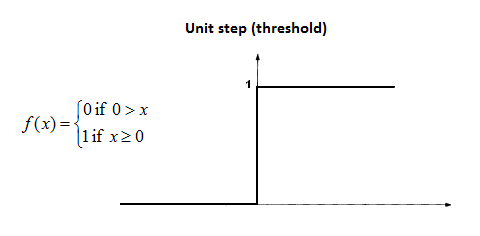
\includegraphics[width=0.5\textwidth]{step-function.png}
\end{figure}

\begin{itemize}
    \item Output is 1 when the value > 0
    \item Output is 0 when the value < 0
    \item Downsides:
    \begin{itemize}
        \item Binary: can only output yes or no (100\% of 0\%)
        \item Problems with multiple classes. What if multiple classes output more than 0?
        \item Hard to train: backpropagation does not work (the derivative is 0)
    \end{itemize}
    \item Use:
    \begin{itemize}
        \item Do not use the step function
    \end{itemize}
\end{itemize}


\subsubsection{Linear function (Adaline)}

\begin{figure}[H]
    \centering
    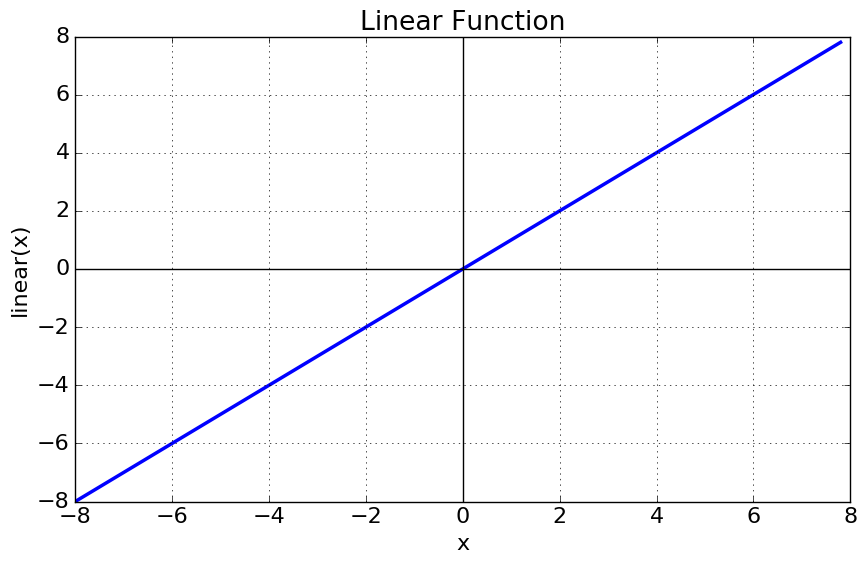
\includegraphics[width=0.4\textwidth]{adaline.png}
\end{figure}

\begin{itemize}
    \item Output is proportional to the input
    \item Downsides:
    \begin{itemize}
        \item It doesn't matter how many layers you use, in the end, the output of stacked lineair layers
        \item The derivative is constant: does not have a relation to the input
    \end{itemize}
    \item Use:
    \begin{itemize}
        \item Input layer
        \item Output layer with regressie
    \end{itemize}
\end{itemize}

\subsubsection{Sigmoid function}

\begin{figure}[H]
    \centering
    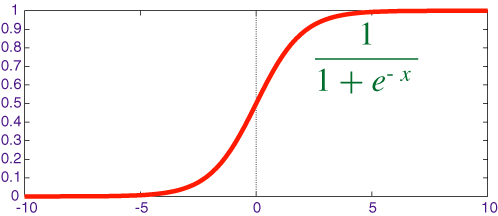
\includegraphics[width=0.4\textwidth]{sigmoid.png}
\end{figure}

\begin{itemize}
    \item Non-linear
    \item The output will always be between 0 and +1
    \item Downsides:
    \begin{itemize}
        \item Vanishing gradient descent has a higher performance than adaptive techniques problem: problematic for neural networks with many hidden layers
    \end{itemize}
    \item Use:
    \begin{itemize}
        \item Is not used that much anymore for hidden layers
        \item Sometimes used for output layer with classification problems
    \end{itemize}
\end{itemize}


\subsubsection{Hyperbolic tangent (tanh)}

\begin{figure}[H]
    \centering
    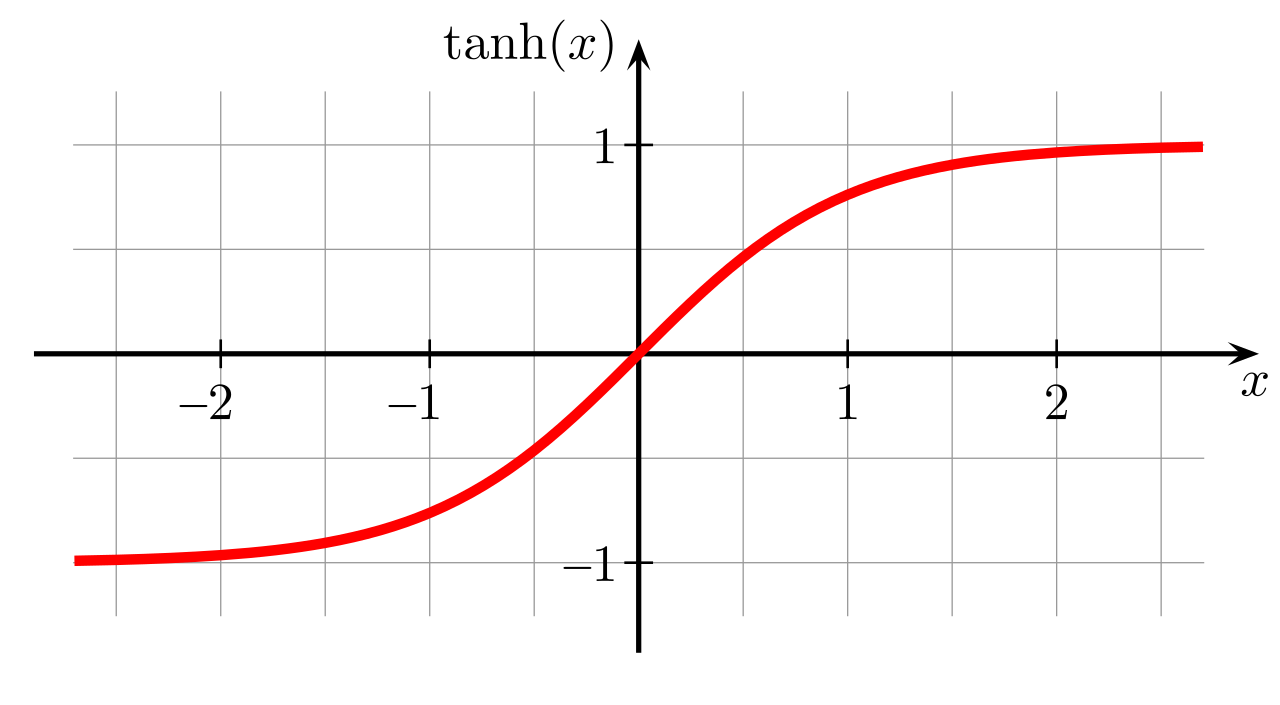
\includegraphics[width=0.4\textwidth]{tanh.png}
\end{figure}


\begin{itemize}
    \item Non-linear
    \item The output is always between -1 and +1
    \item Centered around 0
    \item Downsides:
    \begin{itemize}
        \item Vanishing gradient problem is still present
    \end{itemize}
    \item Use:
    \begin{itemize}
        \item Is not used that much anymore, except for specific architectures
    \end{itemize}
\end{itemize}

\subsubsection{Rectified Linear Unit (ReLu)}

\begin{figure}[H]
    \centering
    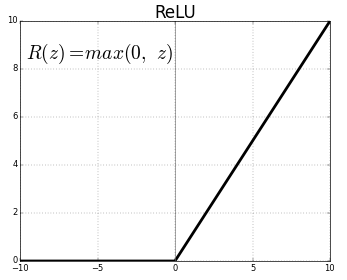
\includegraphics[width=0.35\textwidth]{relu.png}
\end{figure}

\begin{itemize}
    \item Non-linear
    \item Every function can be approached using a combination of ReLu functions
    \item Computationally efficient
    \item Downsides:
    \begin{itemize}
        \item Sparse activation: many activations become 0
        \item $\Rightarrow$ `Dead' neurons cannot be activated again
    \end{itemize}
    \item Use:
    \begin{itemize}
        \item For hidden layers
    \end{itemize}
\end{itemize}


\subsubsection{Leaky ReLu}

\begin{figure}[H]
    \centering
    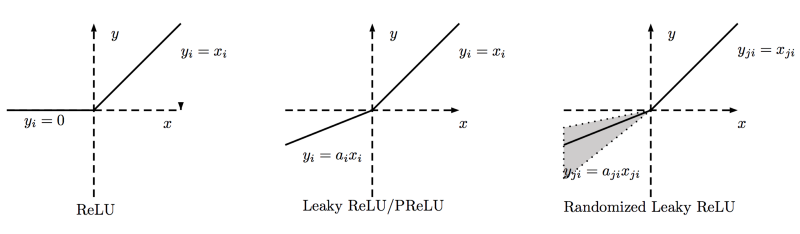
\includegraphics[width=0.7\textwidth]{leaky-relu.png}
\end{figure}


\begin{itemize}
    \item Variant on ReLu
    \item Neurons do not `die': there is still a low gradient when $x < 0$
    \item Downsides:
    \begin{itemize}
        \item More parameters to train
    \end{itemize}
    \item Gebruik:
    \begin{itemize}
        \item For hidden layers
    \end{itemize}
\end{itemize}

\subsubsection{Conclusion}

Hidden layers:

\begin{itemize}
    \item First try ReLu
    \item Try Leaky ReLu
    \item Usually no Sigmoid or Tanh.
\end{itemize}


Output layer:
\begin{itemize}
    \item Lineair for regression problems.
    \item Softmax / Sigmoid for classification problems
\end{itemize}


Softmax is a generalisation of Sigmoid: $\sigma(z)_j = \frac{e^{z_j}}{\sum_{k=1}^K e^{z_k}}$

\subsection{Underfitting and overfitting}


\begin{theorem}[Underfitting]
    Underfitting occurs when an AI can not model the training data, and cannot generalize new data.
    
    \begin{itemize}
        \item The model is too 'simple'
        \item Model with high bias
        \item $\Rightarrow$ the score with training data and the score with test data are both low
    \end{itemize}
\end{theorem}

\begin{theorem}[Overfitting]
    Overfitting occurs when an AI models the training data too well, and cannot generalize new data.
    
    \begin{itemize}
        \item The model is too 'complex'
        \item Random noise in the data gets picked up and remembered by the AI
        \item Model with a high variance
        \item $\Rightarrow$ the score with training data is higher than the score with test data
    \end{itemize}
\end{theorem}

\begin{figure}[H]
    \centering
    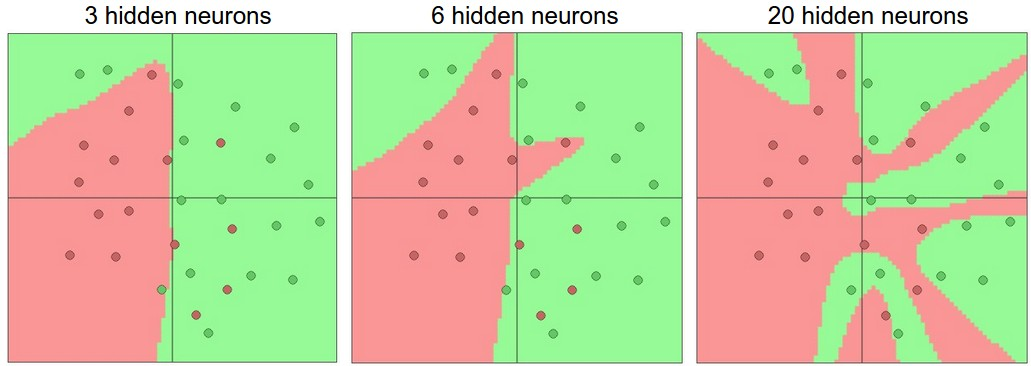
\includegraphics[width=0.5\textwidth]{underfitting-neural.png}
\end{figure}

\begin{itemize}
    \item Too large neural network: overfitting
    \item Too small neural network: underfitting
\end{itemize}

TODO: L1 \& L2 regularization


\subsection{Regularisation}

\begin{theorem}[Regularisation]
Method to find a good balance between underfitting and overfitting.
\end{theorem}

We'll discuss 2 regularisation methods:

\begin{itemize}
    \item Ridge regression (L2 regularisation)
    \item Lasso regression (L1 regularisation)
\end{itemize}

\subsubsection{Regularisation with L2}

TODO

\subsubsection{Regularisation with L1}

TODO

\subsubsection{Dropout}

\begin{figure}[H]
    \centering
    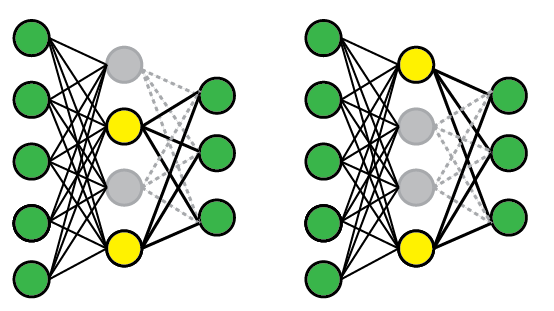
\includegraphics[width=0.35\textwidth]{dropout.png}
\end{figure}

\begin{theorem}
    Dropout (or `Dilution') is a regularisation technique to prevent overfitting in neural networks.
    This happens by disabling a certain percentage of neurons in the network. Other neurons must then take over from the disabled neurons.
\end{theorem}

\begin{itemize}
    \item Randomly switch off a certain percentage of neurons in a layer.
    \item Active neurons have to take over.
    \item Hidden layers are forced to learn the general underlying structure.
    \item Emulates an ensemble of neural networks.
    \item Can be responsible for the fact that the validation accuracy is higher than the training accuracy.
    \item Dropout only happens during training time. When making predictions, the full network is used.
\end{itemize}

\url{https://en.wikipedia.org/wiki/Dilution_(neural_networks)}

\subsubsection{Noise injection}

\begin{theorem}
    Noise injection makes a neural network \textbf{more robust against small changes} in the weights
\end{theorem}

\begin{itemize}
    \item Without noise injection: train(X , Y)
    \item With noise injection: train(X+noise , Y)
\end{itemize}

Instead of adding noise to the input, add noise to the weights w:

$Y = f (X, W + noise), noise ~ N(0, kleine \sigma)$


\subsection{Gradient Descent modes}

\subsubsection{Full gradient descent}

\begin{itemize}
    \item Batch size = full training set
    \item Also called batch mode
    \item Not always suited for large data sets
\end{itemize}


\subsubsection{Stochastic gradient descent}

\begin{itemize}
    \item Minimize the costfunction on a sample by sample basis
    \item Batch size = 1 (training) sample.
    \item In the long term the error will decrease.
    \item The learning curve can be very erratic.
\end{itemize}

\subsubsection{Batch gradient descent (mini-batch)}

\begin{itemize}
    \item Batch size is larger than 1 and smaller than the size of the training set.
    \item Happy medium.
    \item Less erratic than with stochastic gradient descent.
    \item Also called mini-batch.
\end{itemize}

\begin{figure}[H]
    \centering
    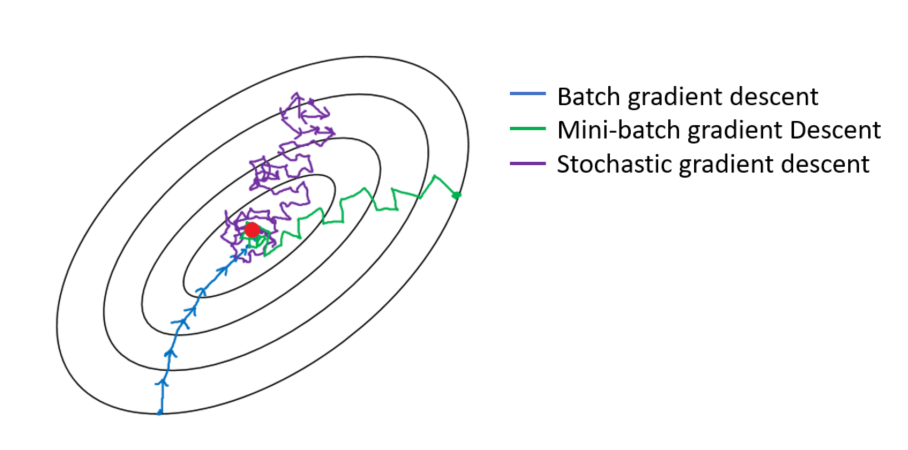
\includegraphics[width=0.65\textwidth]{img/gradient-descent-modes.png}
    \caption{Path of the training loss}
\end{figure}

\begin{figure}[H]
    \centering
    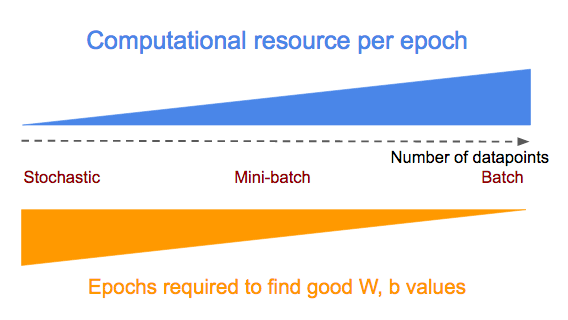
\includegraphics[width=0.5\textwidth]{img/gradient-descent-modes-resources.png}
    \caption{Resources}
\end{figure}

\subsection{Momentum \& adaptive learning rates}

\begin{figure}[H]
    \centering
    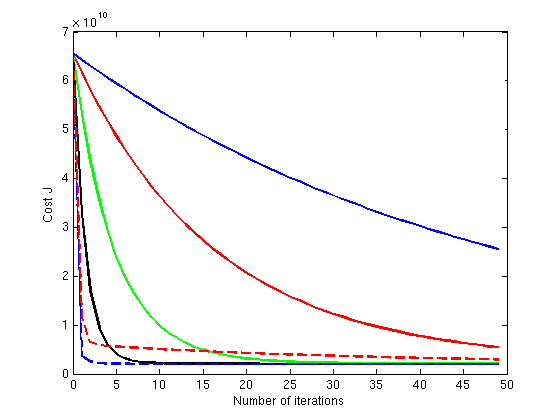
\includegraphics[width=0.5\textwidth]{img/momentum-adaptive-learning-rates.png}
    \caption{TODO}
\end{figure}


\subsubsection{Goal}

\begin{itemize}
    \item speeding up gradient descent.
    \item Momentum is the most important factor
    \begin{itemize}
        \item = The force that keeps an object moving or keeps an event developing after it has started.
        \item Less erratic movements of the training loss.
        \item Updating the weights: $\theta t = \theta t - 1 + \mu v t - 1 - \eta g t$ 
    \end{itemize}
\end{itemize}

\subsubsection{Nesterov momentum}

Make a jump in the direction of the momentum, compute the gradient and adjust the
trajectory.

\begin{figure}[H]
    \centering
    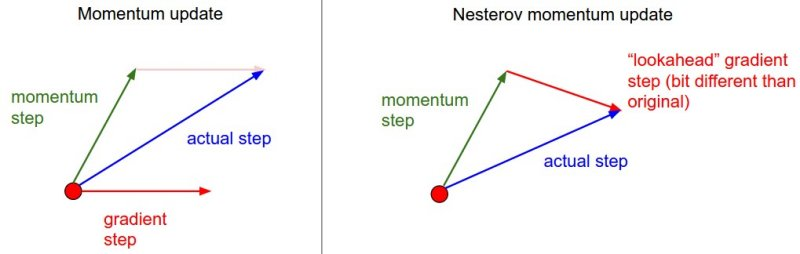
\includegraphics[width=0.5\textwidth]{img/nesterov-momentum.png}
    \caption{Nesterov momentum}
\end{figure}

\subsubsection{Variable learning rates}

\begin{enumerate}
    \item Step Decay:
    \begin{itemize}
        \item Decrease the learning rate every x iterations. 
        \item Example: every 100 iterations the learning is cut in half.
    \end{itemize}
    \item Exponential Decay:
    \begin{itemize}
        \item $\eta(t) = A\cdot e^{-kt}$
    \end{itemize}
    \item 1/t Decay:
    \begin{itemize}
        \item $\eta(t) = \frac{A}{kt + 1}$        
        \item Slower than exponential decay
    \end{itemize}
    \item Babysitting method:
    \begin{itemize}
        \item Train for a couple of epochs and look what's going on. 
        \item If necessary, change the learning rate.
        \item \textbf{Warning:} can be stuck on a plateau
    \end{itemize}
\end{enumerate}

\subsubsection{Adaptive learning rates}

\begin{enumerate}
    \item Adagrad:
    \begin{itemize}
        \item The cost of each parameter (weight) is different: steep in one direction, flat in the other direction.
        \item Adjust the learing rate of each individual parameter based on how much it has been adjusted in the past = cache.
        \item $\theta(t) = \theta(t-1) - \eta \frac{\Delta J}{\sqrt{cache + e}}$
    \end{itemize}
    \item RMSprop:
    \begin{itemize}
        \item Adagrad is too agressive in lowering the learning rate.
        \item Decrease the cache with every update
        \item cache = decay x cache + (1 - decay) x gradient$^2$
        \item Decay is typically $0.99$ or $0.999$
    \end{itemize}
    \item Adam:
    \begin{itemize}
        \item Most popular optimizer in deep learning
        \item Combines RMSprop with momentum
        \item TODO: formulas
        \item \textbf{Remark:} experiments show that regular gradient descent has a higher performance than adaptive techniques
    \end{itemize}
\end{enumerate}

\subsection{Weight initialization}

\begin{itemize}
    \item Observation: the deeper the better. More layers are better than more neurons per layer
    \item Problems of deep learning: vanishing gradients and exploding gradients
\end{itemize}

\begin{figure}[H]
    \centering
    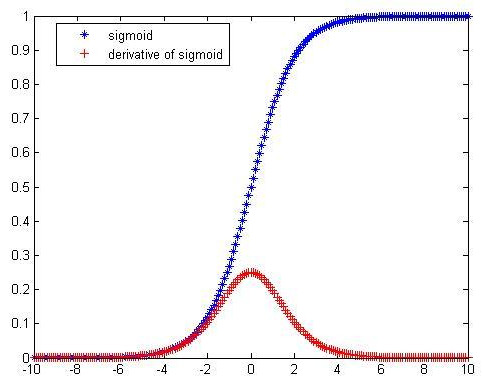
\includegraphics[width=0.5\textwidth]{img/vanishing-exploding-gradient.png}
    \caption{TODO}
\end{figure}

\subsubsection{Solutions to the vanishing gradient and exploding gradient problem}

\begin{itemize}
    \item Greedy layer-wise unsupervised pre-training.
    \item ReLu.
    \item Good initialization of the weights. (random)
\end{itemize}

\subsubsection{Types of initializations}

\begin{enumerate}
    \item Constant: leads to symmetry. Has to be avoided!
    \item Random:
    \begin{itemize}
        \item Uses the np.random functions
        \item Other: Glorot uniform, Lecun (uniform distribution)
        \item Bias can be initialized to 0
    \end{itemize}
\end{enumerate}

\subsection{Batch normalization}

\begin{itemize}
    \item We like to normalize our data.
    \item A lot of activation functions have a limited active range.
    \item Makes sure that each layer learn a bit more independently from the other layers.
    \item Regularization effect: less prone to overfitting.
    \item Adds a small amount of noise to each layer. Less need for dropout.
    \item \textbf{Normalize each layer of the neural network}
\end{itemize}

\begin{figure}[H]
    \centering
    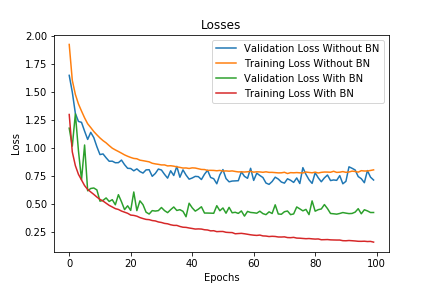
\includegraphics[width=0.5\textwidth]{img/batch-normailzation-training-loss.png}
    \caption{Training loss with \& without batch normailzation}
\end{figure}

\section{Keras}

\subsection{What is Keras}

\begin{itemize}
    \item Neural Network library written in Python.
    \item Built on top of Tensorflow and Theano.
    \item Easy to use.
    \item Modular.
    \item Makes it possible to build complex neural networks
\end{itemize}

\subsection{The sequential model}

\begin{itemize}
    \item Stacking layers on top of each other.
    \item \url{https://keras.io/#getting-started-30-seconds-to-keras}
\end{itemize}

\begin{minted}{python}
import tensorflow as tf
from tf.keras.models import Sequential
model = Sequential()

from tf.keras.layers import Dense, Activation
model.add(Dense(units=30, input_dim=10))
model.add(Activation('relu'))
model.add(Dense(units=5))
model.add(Activation('softmax'))
\end{minted}

$\Rightarrow$ 10 inputs | 30 hidden layer ReLu units | 5 softmax outputs

\subsubsection{Compiling, training and making predictions}

\begin{minted}{python}
model.compile(loss='categorical_crossentropy',
              optimizer='sgd',
              metrics=['accuracy'])

model.compile(loss=keras.losses.categorical_crossentropy,
              optimizer = keras.optimizers.SGD(lr=0.01,momentum=0.9, nesterov=True)
            )
model.fit(x_train, y_train, epochs=5, batch_size=32)
classes = model.predict(x_test, batch_size=128)
\end{minted}

\subsection{Parameters of the sequential model}

\subsubsection{Activation functions}

\url{https://keras.io/activations/}

Available activation functions:

\begin{itemize}
    \item softmax
    \item relu
    \item sigmoid
    \item tanh
    \item linear
    \item \url{https://keras.io/layers/advanced-activations/}
\end{itemize}

\subsubsection{Learning rate optimizers}

\url{https://keras.io/optimizers/}

\begin{itemize}
    \item SGD + Nesterov (Stochastic Gradient Descent)
    \item RMSProp: more applicable to recurrent networks
    \item Adagrad
    \item Adam
    \item Adamax
\end{itemize}

\subsubsection{Loss function}

\url{https://keras.io/losses/#available-loss-functions}

\begin{itemize}
    \item The loss function to be optimized during the training process.
    \item Error losses: (usually for regression)
    \begin{itemize}
        \item mean\_squared\_error(y\_true, y\_pred)
        \item mean\_absolute\_error(y\_true, y\_pred)
        \item mean\_absolute\_percentage\_error(y\_true, y\_pred)
        \item mean\_squared\_logarithmic\_error(y\_true, y\_pred)
    \end{itemize}
    \item Hinge losses: (usually for Support Vector Machines (SVM))
    \begin{itemize}
        \item squared\_hinge(y\_true, y\_pred)
        \item hinge(y\_true, y\_pred)
        \item categorical\_hinge(y\_true, y\_pred)
    \end{itemize}
    \item Class losses: (usually for classification)
    \begin{itemize}
        \item binary\_crossentropy(y\_true, y\_pred)
        \begin{itemize}
            \item for \textbf{binary classification or multilabel classification}: problems where a sample can belong to more than one class
            \item With sigmoid
        \end{itemize}
        \item categorical\_crossentropy(y\_true, y\_pred)
        \begin{itemize}
            \item For \textbf{multiclass classification} with softmax where a data sample can only belong to one class.
            \item With softmax
        \end{itemize}
    \end{itemize}
\end{itemize}

\subsection{Metrics}

Used for performance evaluation

\begin{itemize}
    \item Regression metrics:
    \begin{itemize}
        \item Mean Squared Error: mean\_squared\_error of mse
        \item Mean Absolute Error: mean\_absolute\_error, mae
        \item Mean Absolute Percentage Error: mean\_absolute\_percentage\_error, mape
        \item Cosine Proximity: cosine
    \end{itemize}
    \item Classification metrics:
    \begin{itemize}
        \item Binary Accuracy: binary\_accuracy, acc
        \item Categorical Accuracy: categorical\_accuracy, acc
        \item Top k Categorical Accuracy: top\_k\_categorical\_accuracy
        \item Cosine Proximity
    \end{itemize}
\end{itemize}

\subsection{Hyperparameter tuning}

\begin{itemize}
    \item number of neurons per layer
    \item dropout rate
    \item batchsize
    \item optimizer
    \item weight initialization
    \item learningrate
    \item activation function
    \item loss function
    \item weight decay
    \item \dots
\end{itemize}

We often use Grid Search, Random search and Bayes Optimization to find the best parameters.

\subsection{Imbalanced data}

\subsubsection{Problem of imbalanced data}


\begin{figure}[H]
    \centering
    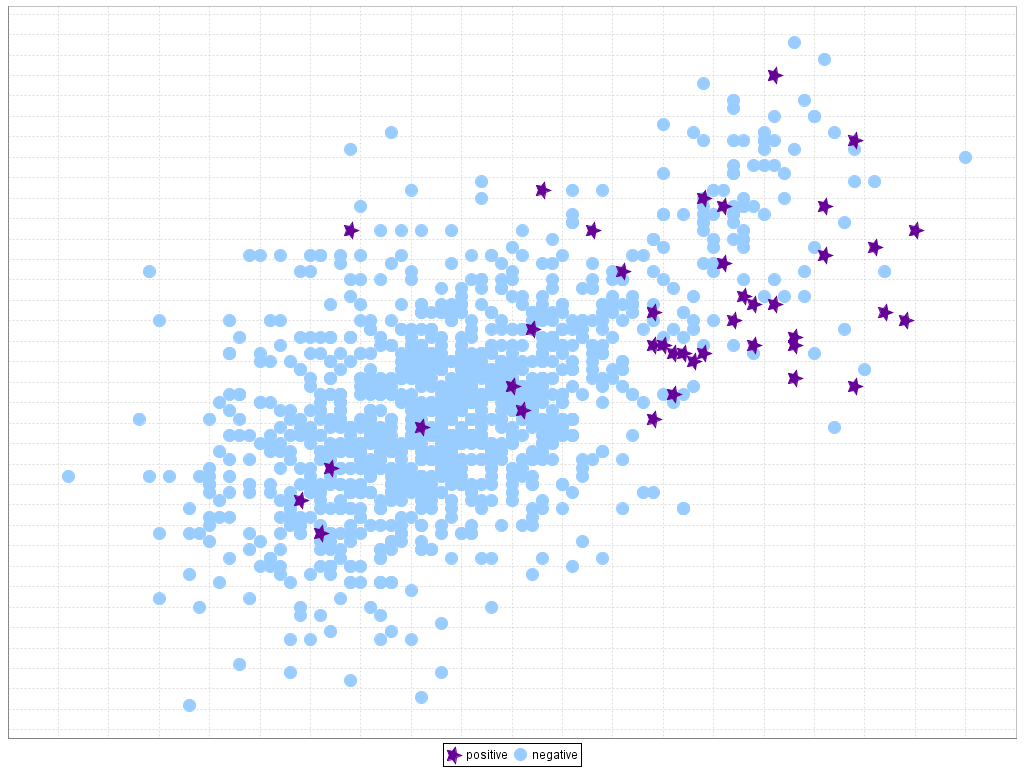
\includegraphics[width=0.4\textwidth]{img/imbalanced-data-problem.png}
    \caption{We have very few data points in the dataset of one class compared to the other}
\end{figure}

\subsubsection{Solutions}

\begin{itemize}
    \item Collect more data
    \item Undersampling \& Oversampling
    \begin{figure}[H]
        \centering
        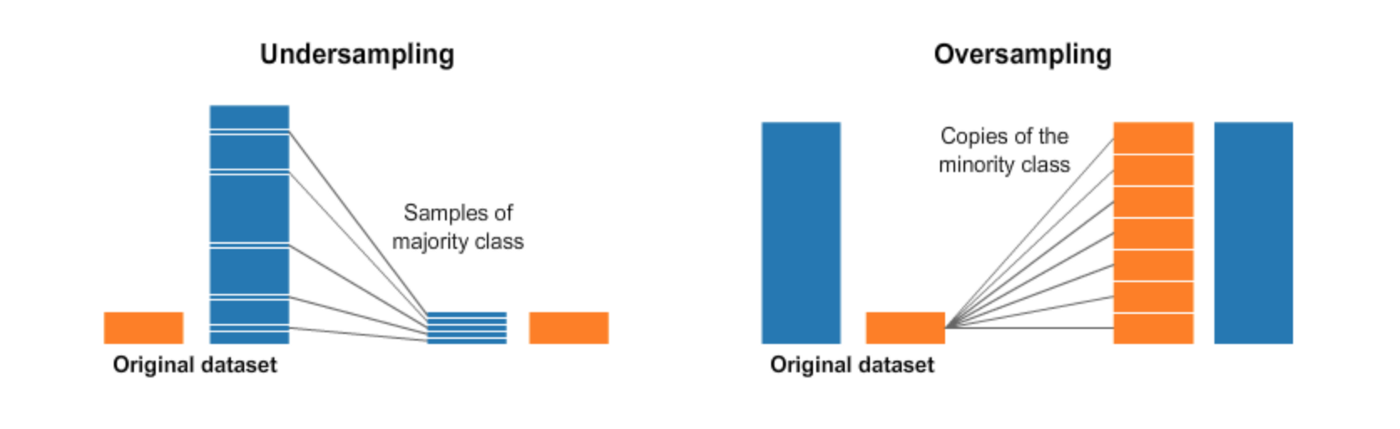
\includegraphics[width=0.7\textwidth]{img/imbalanced-data-sampling.png}
        \caption{Undersampling \& Oversampling}
    \end{figure}
    \item Data augmentation
    \begin{figure}[H]
        \centering
        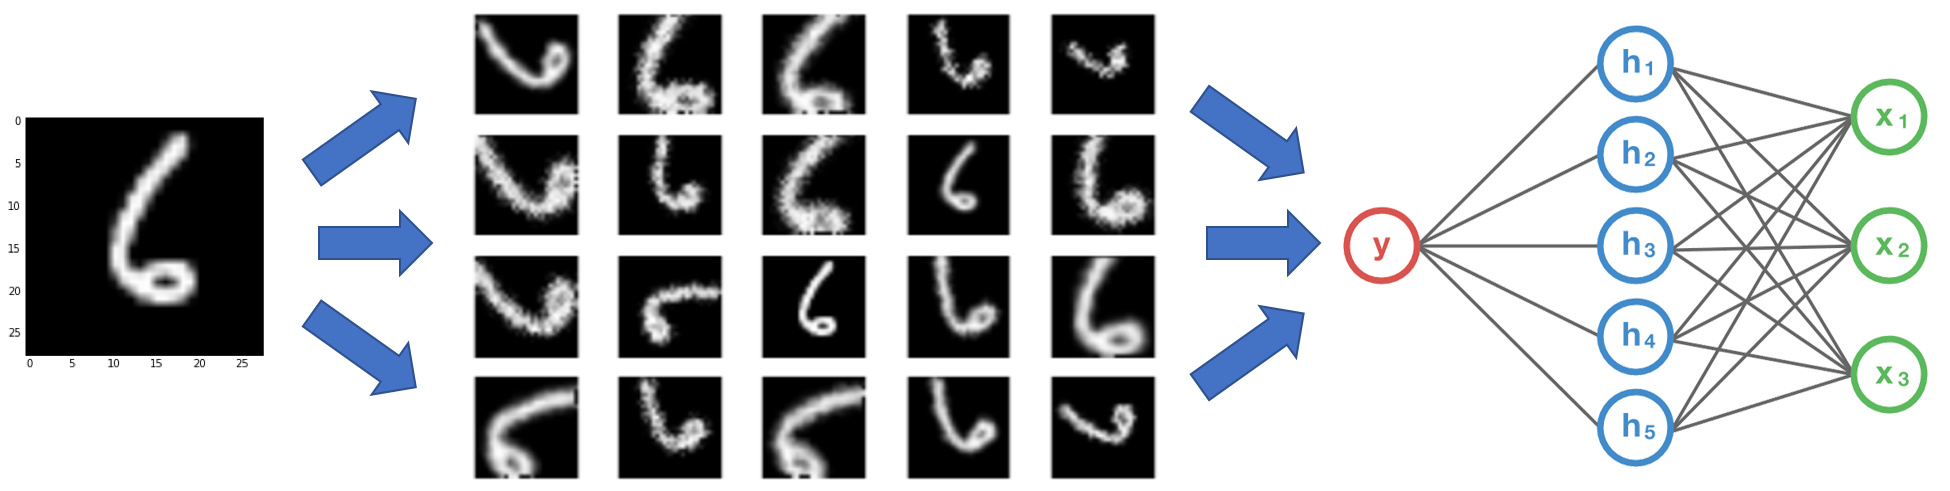
\includegraphics[width=0.5\textwidth]{img/data-augmentation.png}
    \end{figure}
\end{itemize}



\end{document}